\section{\textbf{APPENDIX TEARDROP CURVE}} \label{APPENDIX TEARDROP CURVE}



\subsection       {Plot of Teardrop curve
	[\ref  {01-img-Plot of Teardrop curve.pdf} ] }
\label{ssec-01-img-Plot of Teardrop curve.pdf}

\subsection       {Teardrop Radius of Curvature
	[\ref      {02-img-Teardrop Radius of Curvature.pdf}] }
\label{ssec-02-img-Teardrop Radius of Curvature.pdf}

\subsection       {Teardrop Validation in LinuxCNC
	[\ref      {03-img-Teardrop-Validation-in-LinuxCNC.png} ] }
\label{ssec-03-img-Teardrop-Validation-in-LinuxCNC.png}

\subsection     {Teardrop Direction of Travel 3D
	[\ref      {04-img-Teardrop Direction of Travel 3D.pdf} ] }
\label{ssec-04-img-Teardrop Direction of Travel 3D.pdf}

\subsection       {Teardrop First and Second Order Taylor's Approx
	[\ref      {05-img-Teardrop-First-and-Second-Order-Taylors-Approx.pdf}] }
\label{ssec-05-img-Teardrop-First-and-Second-Order-Taylors-Approx.pdf}

\subsection       {Teardrop First minus Second Order Taylor's Approx
	[\ref      {06-img-Teardrop-First-minus-Second-Order-Taylors-Approx.pdf}] }
\label{ssec-06-img-Teardrop-First-minus-Second-Order-Taylors-Approx.pdf}

\subsection       {Teardrop Separate First Second Order Taylor's Approx
	[\ref      {07-img-Teardrop-Separation-First-and-Second-Order-Taylors-Approx.pdf} ] }
\label{ssec-07-img-Teardrop-Separation-First-and-Second-Order-Taylors-Approx.pdf}

\subsection       {Teardrop Separation SAL and SCL
	[\ref      {08-img-Teardrop-Separation-SAL-and-SCL.pdf}] }
\label{ssec-08-img-Teardrop-Separation-SAL-and-SCL.pdf}

\subsection       {Teardrop Chord-error in close view 2 scales
	[\ref      {09-img-Teardrop-Chord-error-in-close-view-2-scales.pdf}] }
\label{ssec-09-img-Teardrop-Chord-error-in-close-view-2-scales.pdf}

\subsection       {Teardrop Four Components Feedrate Limit
	[\ref      {10-img-Teardrop-Four-Components-Feedrate-Limit.pdf} ] }
\label{ssec-10-img-Teardrop-Four-Components-Feedrate-Limit.pdf}

\subsection    {Teardrop FrateCommand FrateLimit and Curr-Frate
	[\ref      {11-img-Teardrop-FrateCommand-FrateLimit-and-Curr-Frate.pdf}] }
\label{ssec-11-img-Teardrop-FrateCommand-FrateLimit-and-Curr-Frate.pdf}

\subsection     {Teardrop FeedRateLimit minus CurrFeedRate
	[\ref      {12-img-Teardrop-FeedRateLimit-minus-CurrFeedRate.pdf} ] }
\label{ssec-12-img-Teardrop-FeedRateLimit-minus-CurrFeedRate.pdf}

\subsection     {Teardrop FC20-Nominal X and Y Feedrate Profiles
	[\ref      {13-img-Teardrop-FC20-Nominal-X-and-Y-Feedrate-Profiles.pdf} ] }
\label{ssec-13-img-Teardrop-FC20-Nominal-X-and-Y-Feedrate-Profiles.pdf}

\subsection     {Teardrop FC20 Nominal Tangential Acceleration
	[\ref      {14-img-Teardrop-FC20-Nominal-Tangential-Acceleration.pdf} ] }
\label{ssec-14-img-Teardrop-FC20-Nominal-Tangential-Acceleration.pdf}

\subsection     {Teardrop FC20 Nominal Rising S-Curve Profile
	[\ref      {15-img-Teardrop-FC20-Nominal-Rising-S-Curve-Profile.pdf} ] }
\label{ssec-15-img-Teardrop-FC20-Nominal-Rising-S-Curve-Profile.pdf}

\subsection     {Teardrop FC20 Nominal Falling S-Curve Profile
	[\ref      {16-img-Teardrop-FC20-Nominal-Falling-S-Curve-Profile.pdf}] }
\label{ssec-16-img-Teardrop-FC20-Nominal-Falling-S-Curve-Profile.pdf}

\subsection       {Teardrop FC10 Colored Feedrate Profile data ngcode
	[\ref      {17-img-Teardrop-FC10-Colored-Feedrate-Profile-data_ngcode.png} ] }
\label{ssec-17-img-Teardrop-FC10-Colored-Feedrate-Profile-data_ngcode.png}

\subsection       {Teardrop FC20 Colored Feedrate Profile data ngcode
	[\ref      {18-img-Teardrop-FC20-Colored-Feedrate-Profile-data_ngcode.png} ] }
\label{ssec-18-img-Teardrop-FC20-Colored-Feedrate-Profile-data_ngcode.png}

Continue ...\\

\subsection       {Teardrop FC30 Colored Feedrate Profile data ngcode
	[\ref      {19-img-Teardrop-FC30-Colored-Feedrate-Profile-data_ngcode.png} ] }
\label{ssec-19-img-Teardrop-FC30-Colored-Feedrate-Profile-data_ngcode.png}

\subsection       {Teardrop FC40 Colored Feedrate Profile data ngcode
	[\ref      {20-img-Teardrop-FC40-Colored-Feedrate-Profile-data_ngcode.png} ] }
\label{ssec-20-img-Teardrop-FC40-Colored-Feedrate-Profile-data_ngcode.png}

\subsection       {Teardrop FC10 Tangential Acceleration
	[\ref      {21-img-Teardrop-FC10-Tangential-Acceleration.pdf}] }
\label{ssec-21-img-Teardrop-FC10-Tangential-Acceleration.pdf}

\subsection       {Teardrop FC20 Tangential Acceleration
	[\ref      {22-img-Teardrop-FC20-Tangential-Acceleration.pdf}] }
\label{ssec-22-img-Teardrop-FC20-Tangential-Acceleration.pdf}

\subsection       {Teardrop FC30 Tangential Acceleration
	[\ref      {23-img-Teardrop-FC30-Tangential-Acceleration.pdf}] }
\label{ssec-23-img-Teardrop-FC30-Tangential-Acceleration.pdf}

\subsection       {Teardrop FC40 Tangential Acceleration
	[\ref      {24-img-Teardrop-FC40-Tangential-Acceleration.pdf}] }
\label{ssec-24-img-Teardrop-FC40-Tangential-Acceleration.pdf}

\subsection       {Teardrop FC20 Nominal Separation NAL and NCL
	[\ref      {25-img-Teardrop-FC20-Nominal-Separation-NAL-and-NCL.pdf}] }
\label{ssec-25-img-Teardrop-FC20-Nominal-Separation-NAL-and-NCL.pdf}

\subsection       {Teardrop SAL minus SCL for FC10 FC20 FC30 FC40
	[\ref      {26-img-Teardrop-Difference-SAL-minus-SCL-for-FC10-FC20-FC30-FC40.pdf}] }
\label{ssec-26-img-Teardrop-Difference-SAL-minus-SCL-for-FC10-FC20-FC30-FC40.pdf}


\subsection       {Teardrop FC10 FrateCmd CurrFrate X-Frate Y-Frate
	[\ref      {27-img-Teardrop-FC10-FrateCmd-CurrFrate-X-Frate-Y-Frate.pdf}] }
\label{ssec-27-img-Teardrop-FC10-FrateCmd-CurrFrate-X-Frate-Y-Frate.pdf}

\subsection       {Teardrop FC20 FrateCmd CurrFrate X-Frate Y-Frate
	[\ref      {28-img-Teardrop-FC20-FrateCmd-CurrFrate-X-Frate-Y-Frate.pdf}] }
\label{ssec-28-img-Teardrop-FC20-FrateCmd-CurrFrate-X-Frate-Y-Frate.pdf}

\subsection       {Teardrop FC30 FrateCmd CurrFrate X-Frate Y-Frate
	[\ref      {29-img-Teardrop-FC30-FrateCmd-CurrFrate-X-Frate-Y-Frate.pdf}] }
\label{ssec-29-img-Teardrop-FC30-FrateCmd-CurrFrate-X-Frate-Y-Frate.pdf}

\subsection       {Teardrop FC40 FrateCmd CurrFrate X-Frate Y-Frate
	[\ref      {30-img-Teardrop-FC40-FrateCmd-CurrFrate-X-Frate-Y-Frate.pdf}] }
\label{ssec-30-img-Teardrop-FC40-FrateCmd-CurrFrate-X-Frate-Y-Frate.pdf}

\subsection       {Teardrop FC10 Four Components FeedrateLimit
	[\ref      {31-img-Teardrop-FC10-Four-Components-FeedrateLimit.pdf}] }
\label{ssec-31-img-Teardrop-FC10-Four-Components-FeedrateLimit.pdf}

\subsection       {Teardrop FC20 Four Components FeedrateLimit
	[\ref      {32-img-Teardrop-FC20-Four-Components-FeedrateLimit.pdf}] }
\label{ssec-32-img-Teardrop-FC20-Four-Components-FeedrateLimit.pdf}

\subsection       {Teardrop FC30 Four Components FeedrateLimit
	[\ref      {33-img-Teardrop-FC30-Four-Components-FeedrateLimit.pdf}] }
\label{ssec-33-img-Teardrop-FC30-Four-Components-FeedrateLimit.pdf}

\subsection       {Teardrop FC40 Four Components FeedrateLimit
	[\ref      {34-img-Teardrop-FC40-Four-Components-FeedrateLimit.pdf}]}
\label{ssec-34-img-Teardrop-FC40-Four-Components-FeedrateLimit.pdf}

\subsection       {Teardrop Histogram Points FC10 FC20 FC30 FC40
	[\ref      {35-img-Teardrop-Histogram-Points-FC10-FC20-FC30-FC40.pdf}] }
\label{ssec-35-img-Teardrop-Histogram-Points-FC10-FC20-FC30-FC40.pdf}

\subsection    {Teardrop Table distribution of interpolated points
	[\ref      {tab-Teardrop Table distribution of interpolated points}] }
\label{ssec-tab-Teardrop Table distribution of interpolated points}

\subsection         {Teardrop Table FC10-20-30-40 Run Performance data
	[\ref      {tab-app4-Teardrop-Table-FC10-20-30-40-Run-Performance-data}] }
\label{ssec-tab-app4-Teardrop-Table-FC10-20-30-40-Run-Performance-data}


%% =====================================================
%% =====================================================
\clearpage
\pagebreak

\begin{figure}
	\caption     {Plot of Teardrop curve}
	\label{01-img-Plot of Teardrop curve.pdf}
	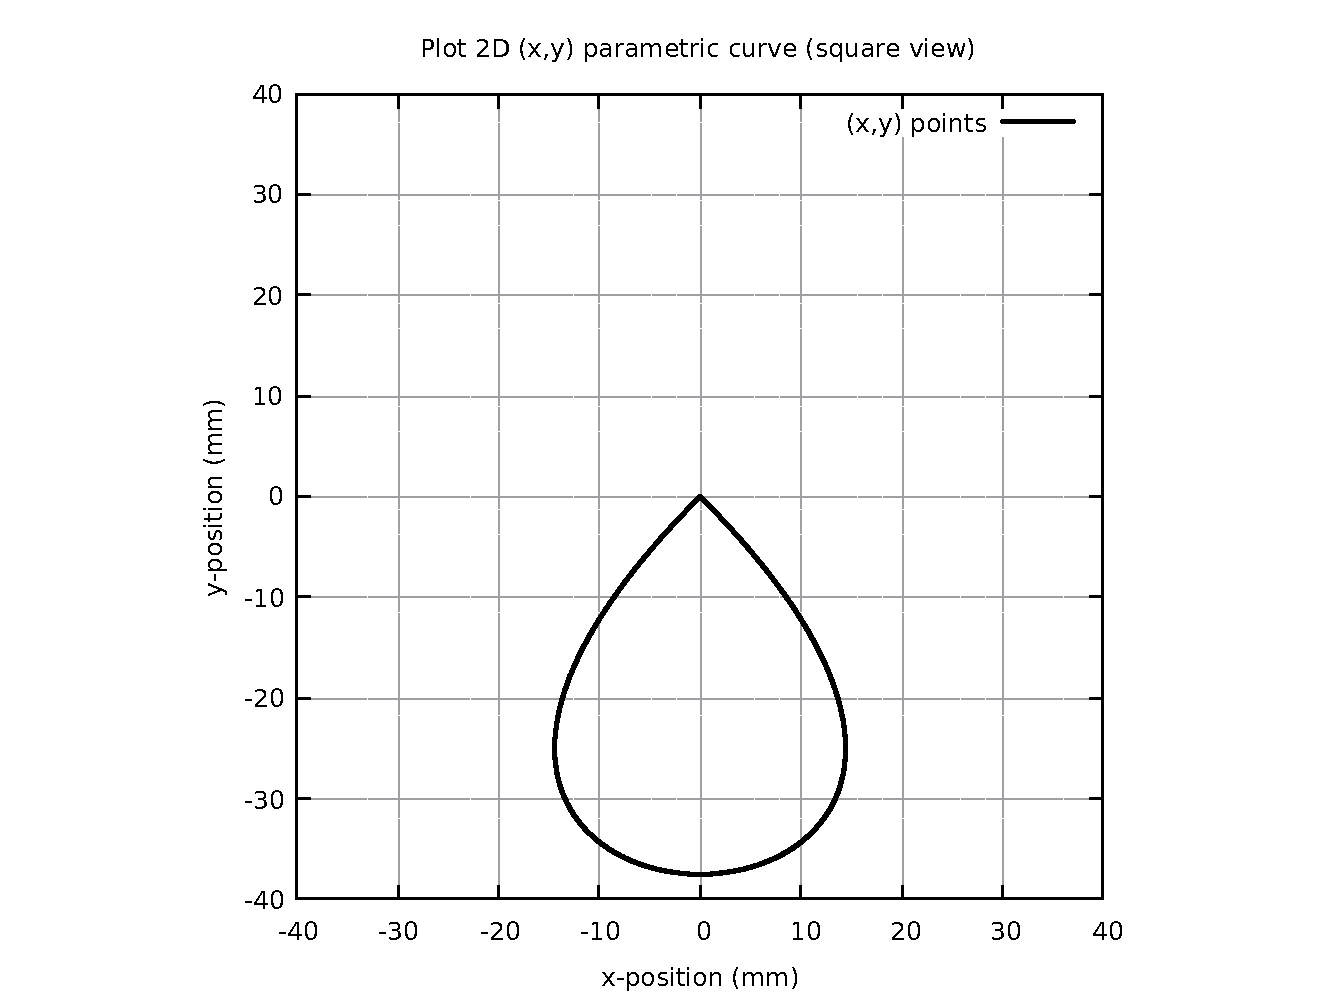
\includegraphics[width=1.00\textwidth]{Chap4/appendix/app-Teardrop/plots/01-img-Plot of Teardrop curve.pdf}
\end{figure}	


\begin{figure}
	\caption     {Teardrop Radius of Curvature}
	\label{02-img-Teardrop Radius of Curvature.pdf}
	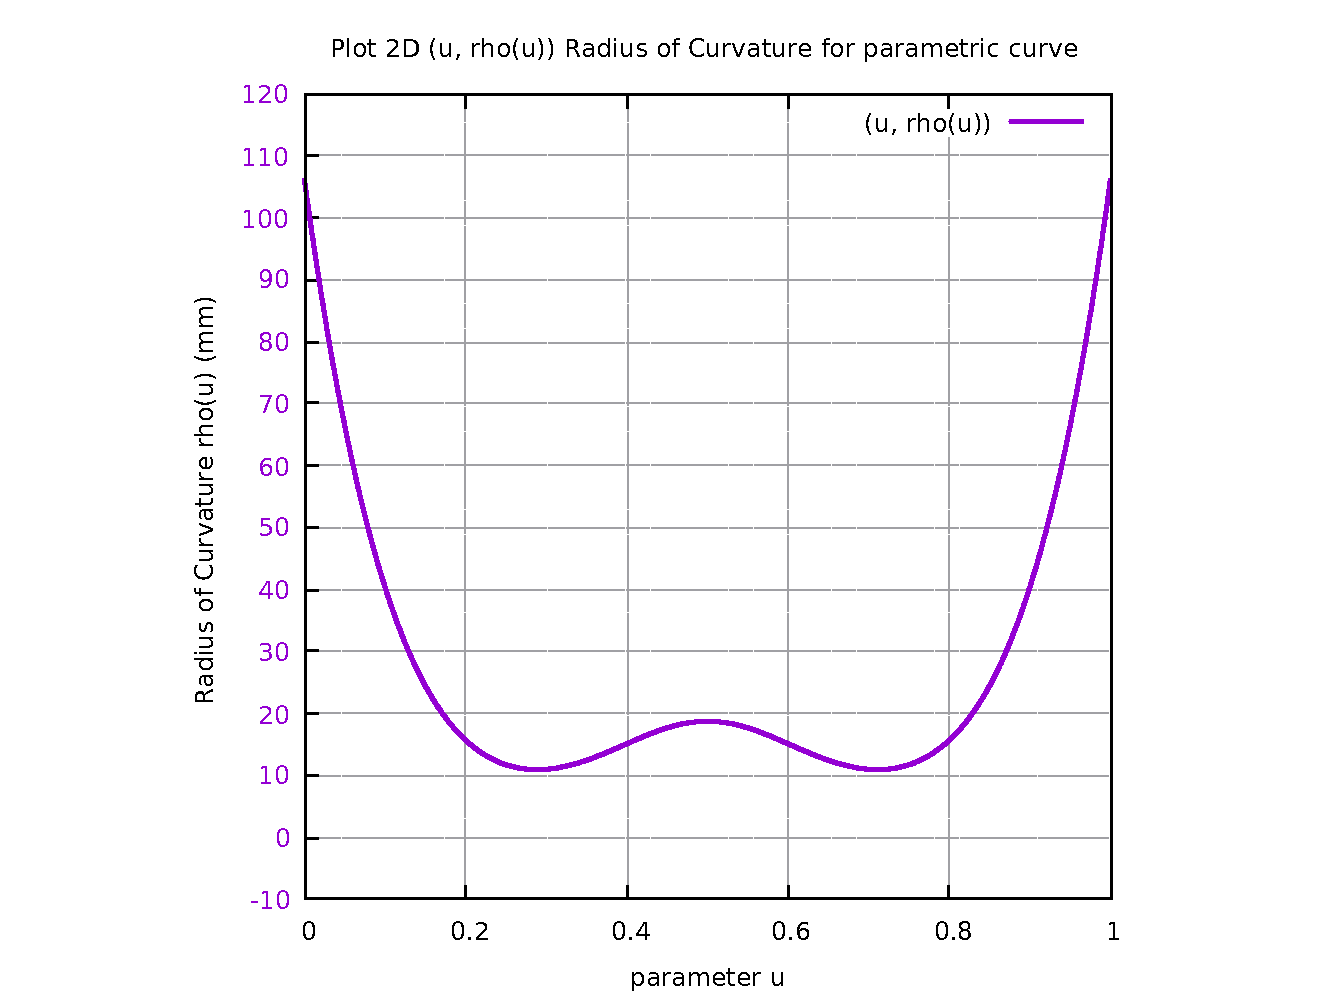
\includegraphics[width=1.00\textwidth]{Chap4/appendix/app-Teardrop/plots/02-img-Teardrop Radius of Curvature.pdf} 
\end{figure}	


%% ==================================================
\clearpage
\pagebreak

\begin{figure}
	\caption     {Teardrop Validation in LinuxCNC}
	\label{03-img-Teardrop-Validation-in-LinuxCNC.png}
	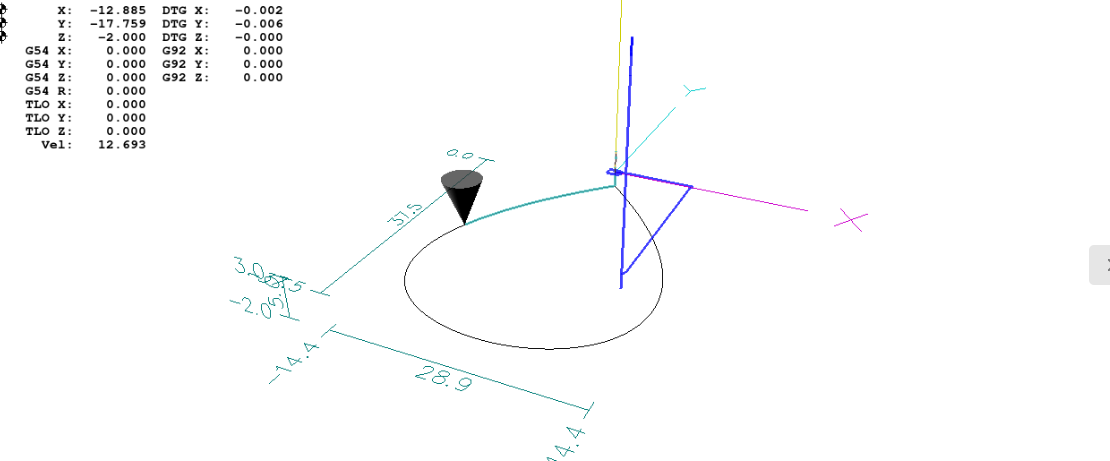
\includegraphics[width=1.00\textwidth]{Chap4/appendix/app-Teardrop/plots/03-img-Teardrop-Validation-in-LinuxCNC.png}
\end{figure}


\begin{figure}
	\caption     {Teardrop Direction of Travel 3D}
	\label{04-img-Teardrop Direction of Travel 3D.pdf}
	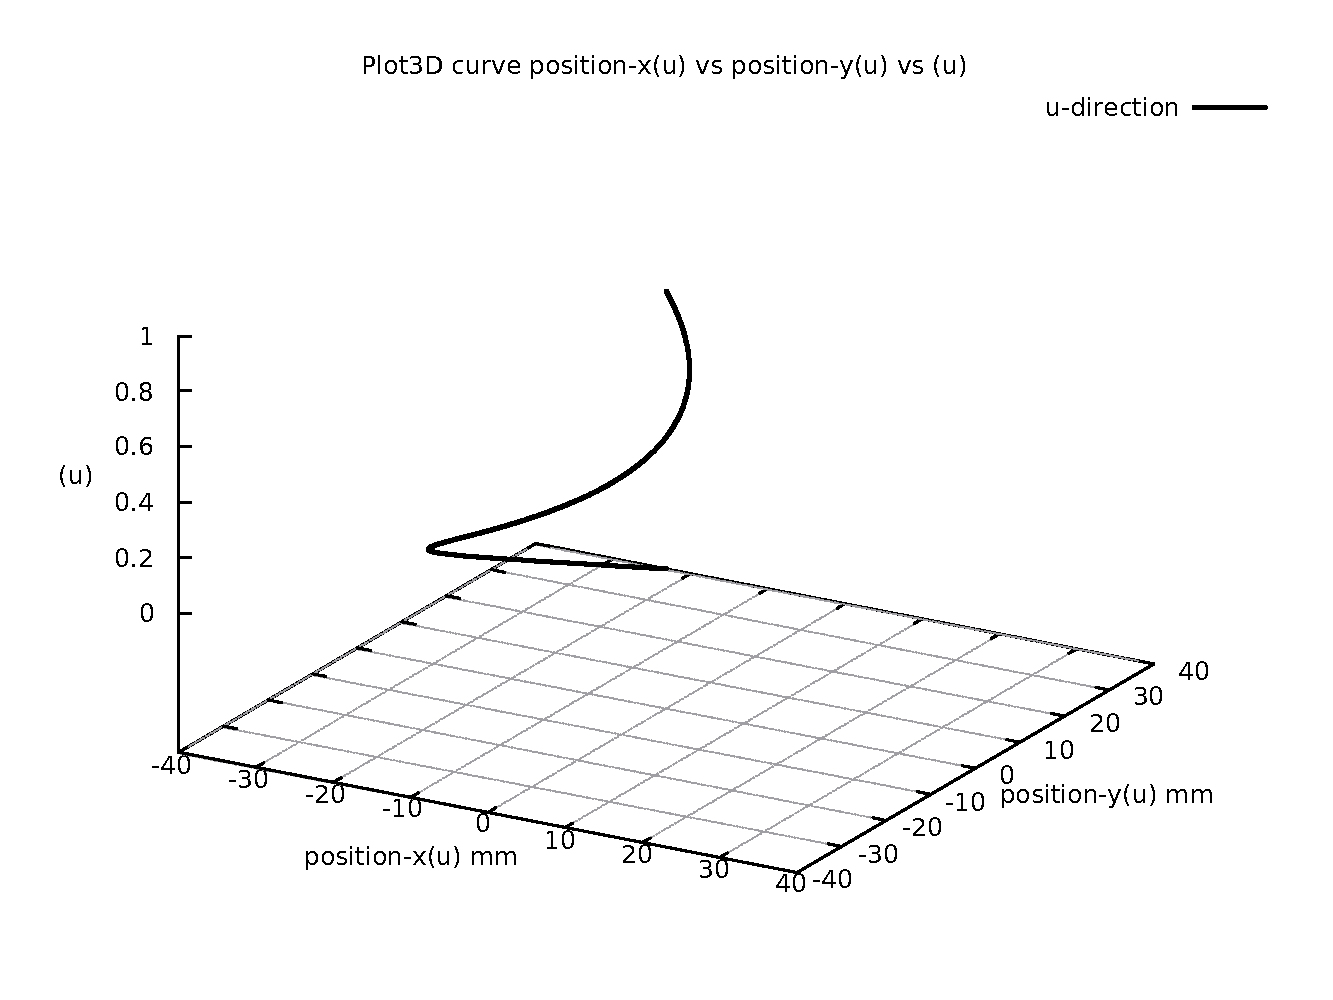
\includegraphics[width=1.00\textwidth]{Chap4/appendix/app-Teardrop/plots/04-img-Teardrop Direction of Travel 3D.pdf}
\end{figure}

%% ==================================================
\clearpage
\pagebreak

\begin{figure}
	\caption     {Teardrop First and Second Order Taylor's Approximation}
	\label{05-img-Teardrop-First-and-Second-Order-Taylors-Approx.pdf}
	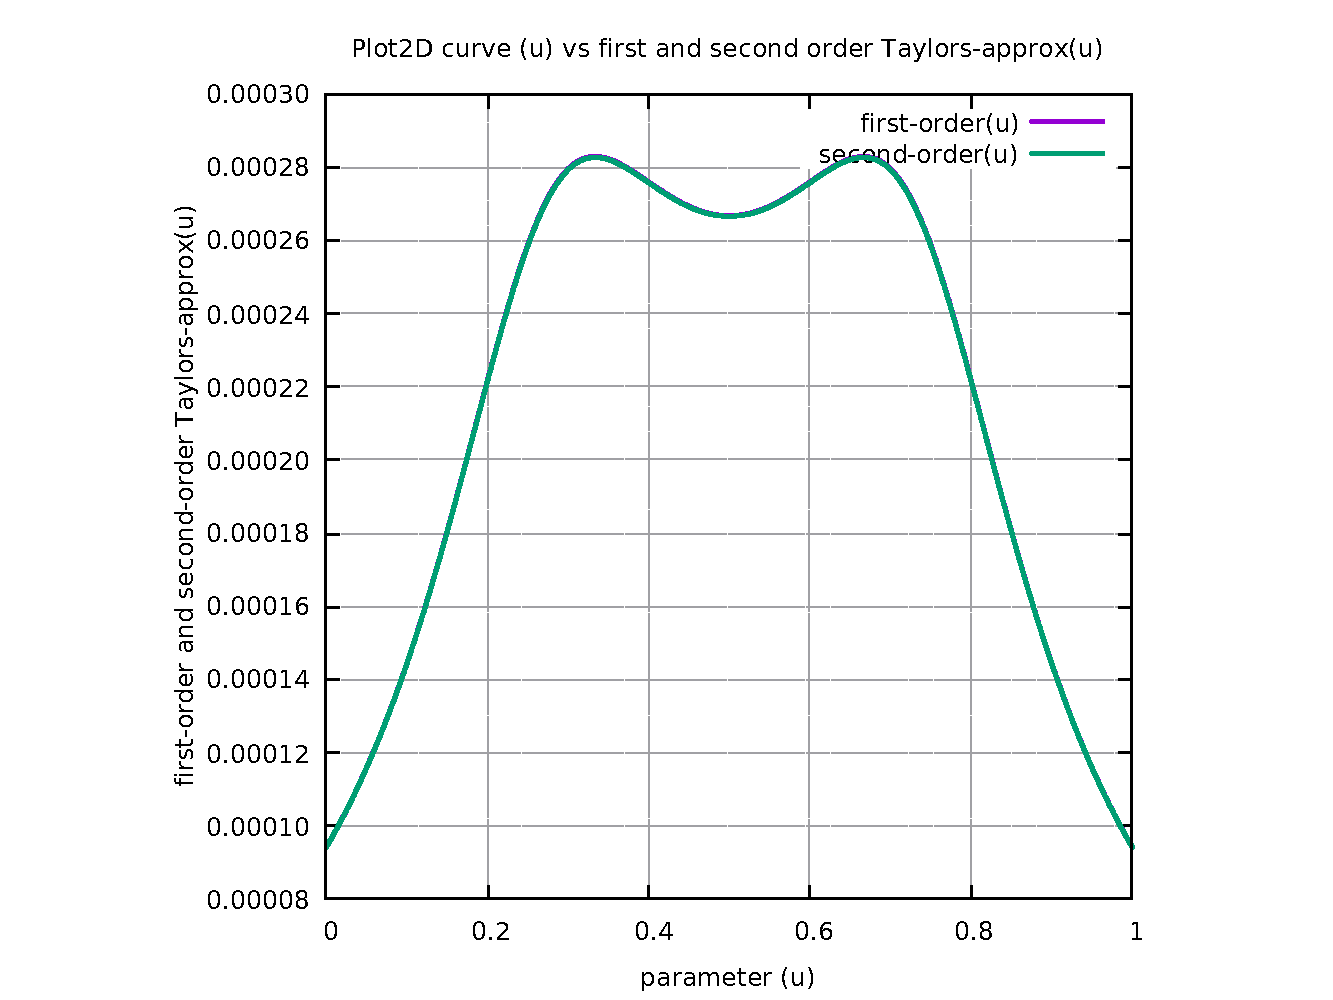
\includegraphics[width=1.00\textwidth]{Chap4/appendix/app-Teardrop/plots/05-img-Teardrop-First-and-Second-Order-Taylors-Approx.pdf}
\end{figure}


\begin{figure}
	\caption     {Teardrop First minus Second Order Taylor's Approximation}
	\label{06-img-Teardrop-First-minus-Second-Order-Taylors-Approx.pdf}
	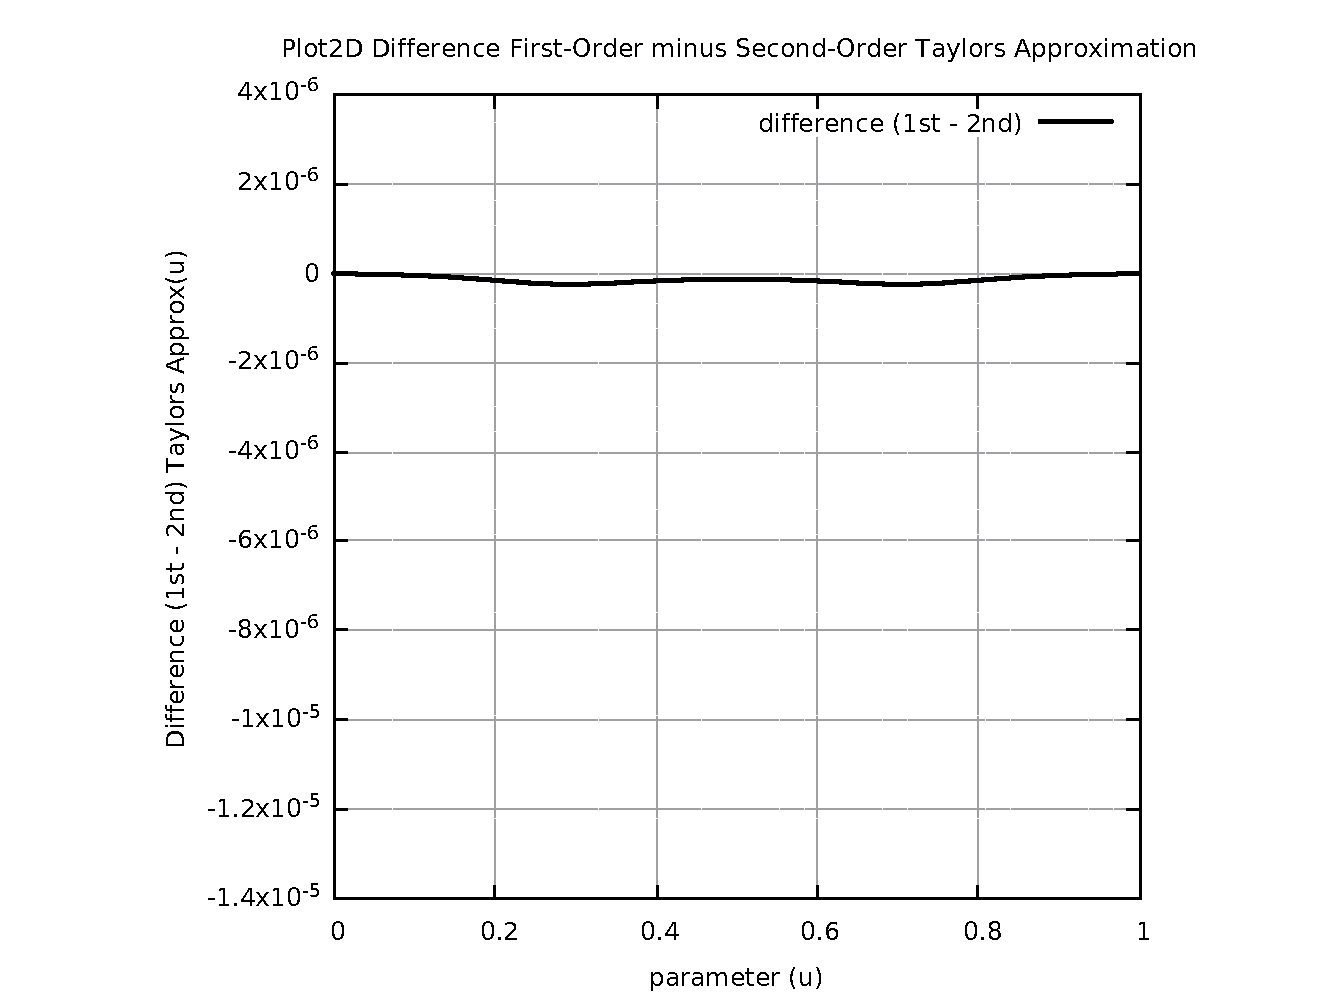
\includegraphics[width=1.00\textwidth]{Chap4/appendix/app-Teardrop/plots/06-img-Teardrop-First-minus-Second-Order-Taylors-Approx.pdf}
\end{figure}

%% ==================================================
\clearpage
\pagebreak

\begin{figure}
	\caption     {Teardrop Separation First and Second Order Taylor's Approximation}
	\label{07-img-Teardrop-Separation-First-and-Second-Order-Taylors-Approx.pdf}
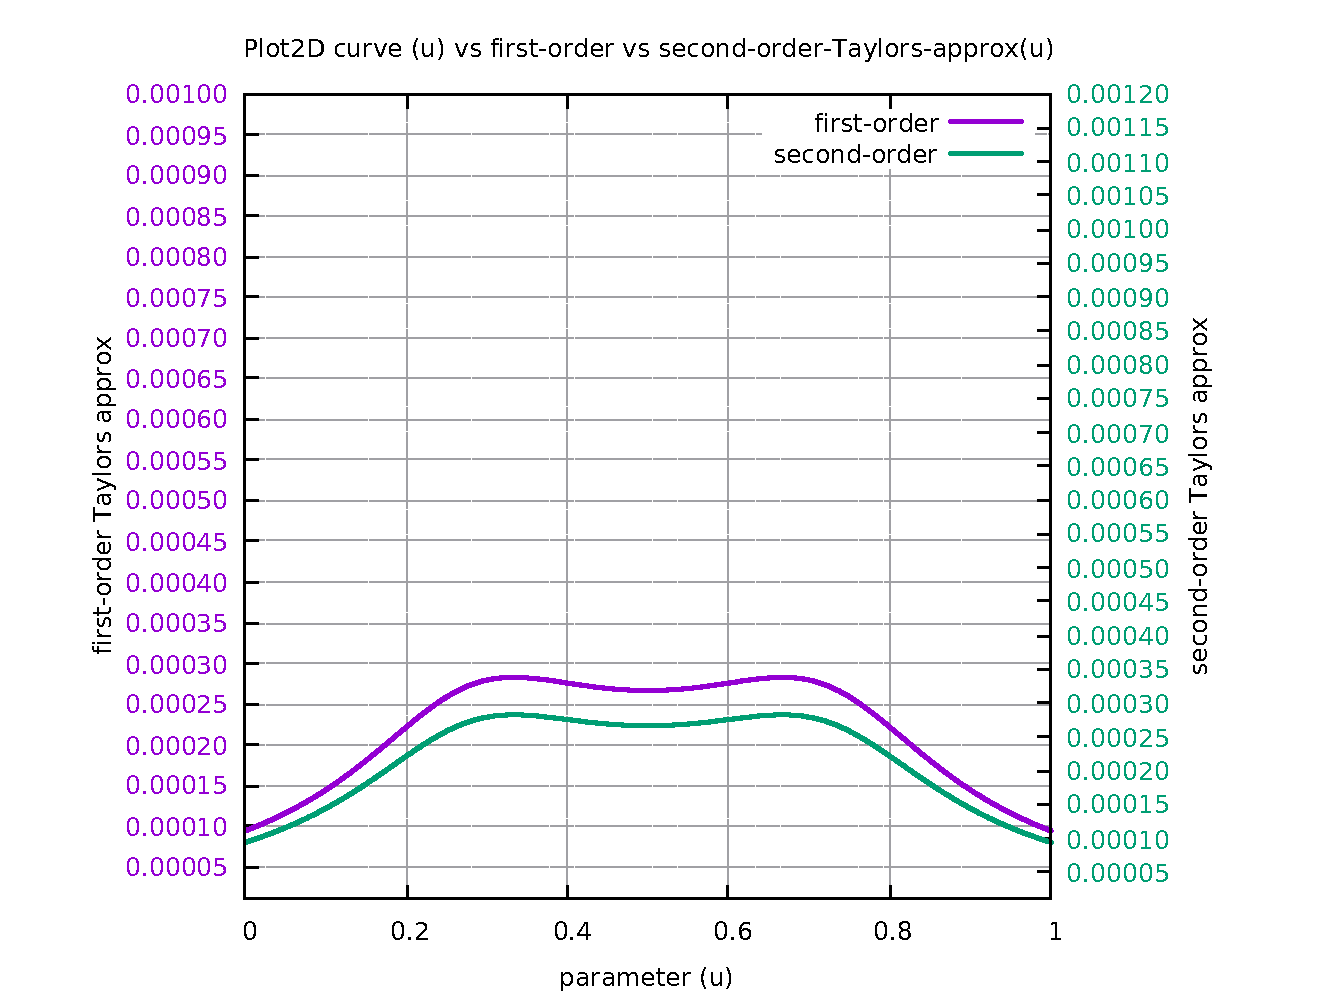
\includegraphics[width=1.00\textwidth]{Chap4/appendix/app-Teardrop/plots/07-img-Teardrop-First-and-Second-Order-Taylors-Approx.pdf}
\end{figure}


\begin{figure}
	\caption     {Teardrop Separation SAL and SCL}
	\label{08-img-Teardrop-Separation-SAL-and-SCL.pdf}
	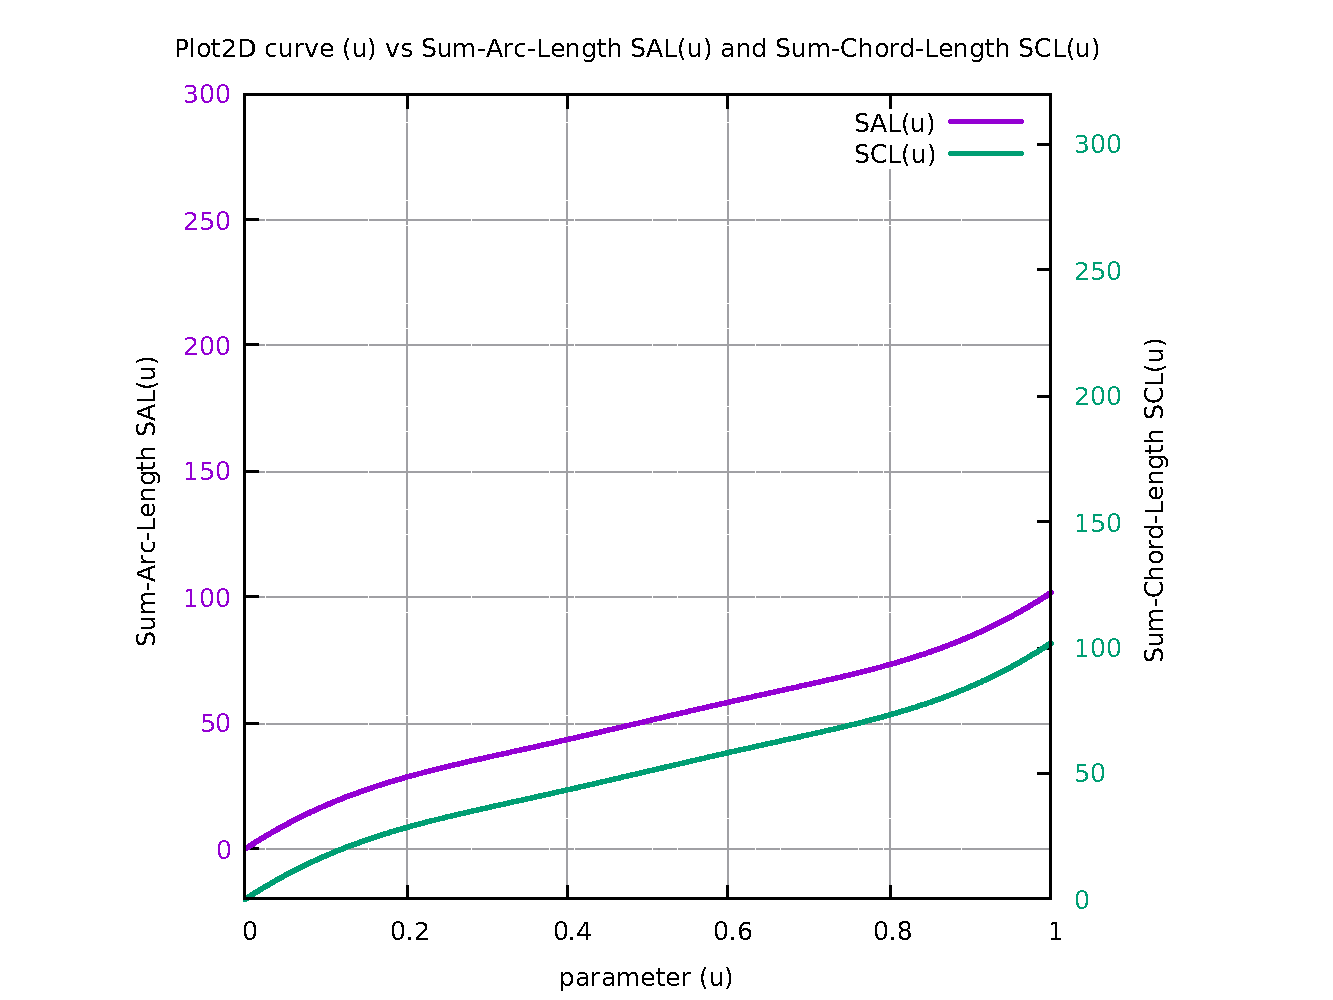
\includegraphics[width=1.00\textwidth]{Chap4/appendix/app-Teardrop/plots/08-img-Teardrop-Separation-SAL-and-SCL.pdf}
\end{figure}

%% ==================================================
\clearpage
\pagebreak

\begin{figure}
	\caption     {Teardrop Chord-error in close view 2 scales}
	\label{09-img-Teardrop-Chord-error-in-close-view-2-scales.pdf}
	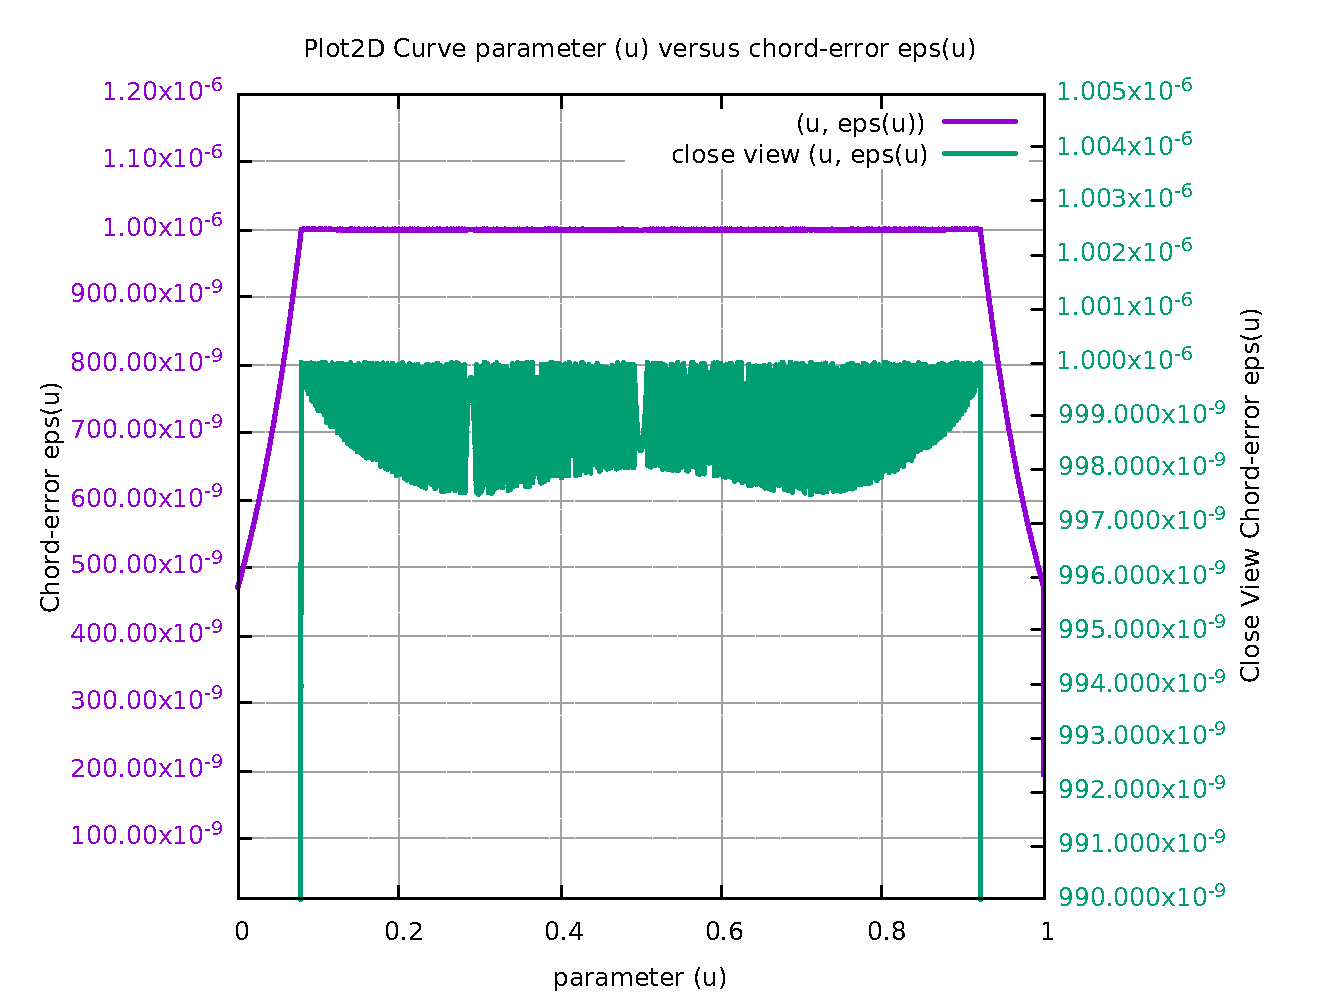
\includegraphics[width=1.00\textwidth]{Chap4/appendix/app-Teardrop/plots/09-img-Teardrop-Chord-error-in-close-view-2-scales.pdf}
\end{figure}

\begin{figure}
	\caption     {Teardrop Four Components Feedrate Limit}
	\label{10-img-Teardrop-Four-Components-Feedrate-Limit.pdf}
	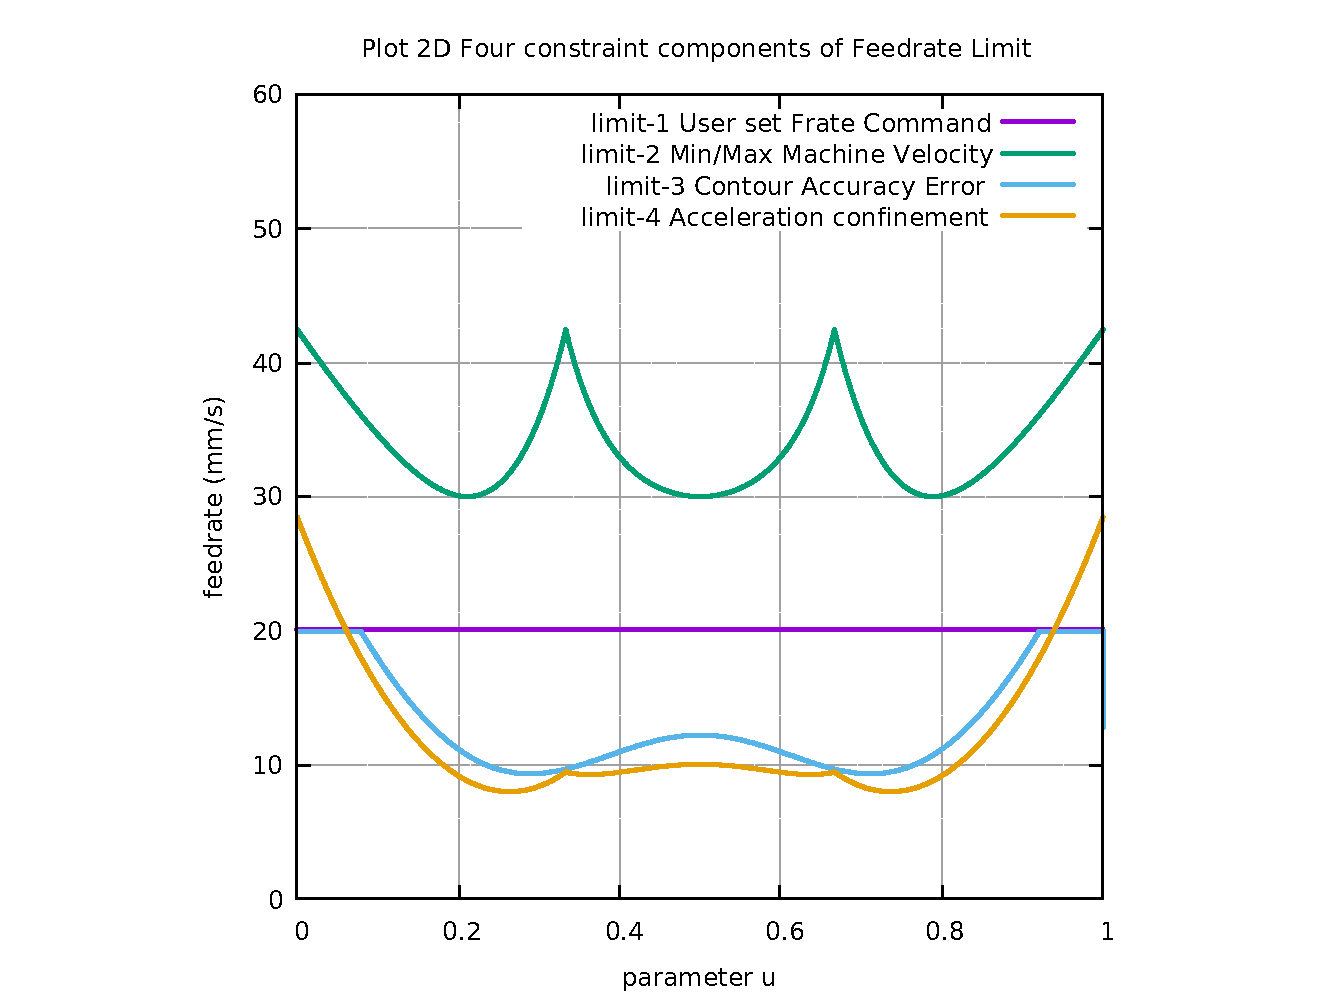
\includegraphics[width=1.00\textwidth]{Chap4/appendix/app-Teardrop/plots/10-img-Teardrop-Four-Components-Feedrate-Limit.pdf}
\end{figure}

%% ==================================================
\clearpage
\pagebreak

\begin{figure}
	\caption     {Teardrop FrateCommand FrateLimit and Curr-Frate}
	\label{11-img-Teardrop-FrateCommand-FrateLimit-and-Curr-Frate.pdf}
	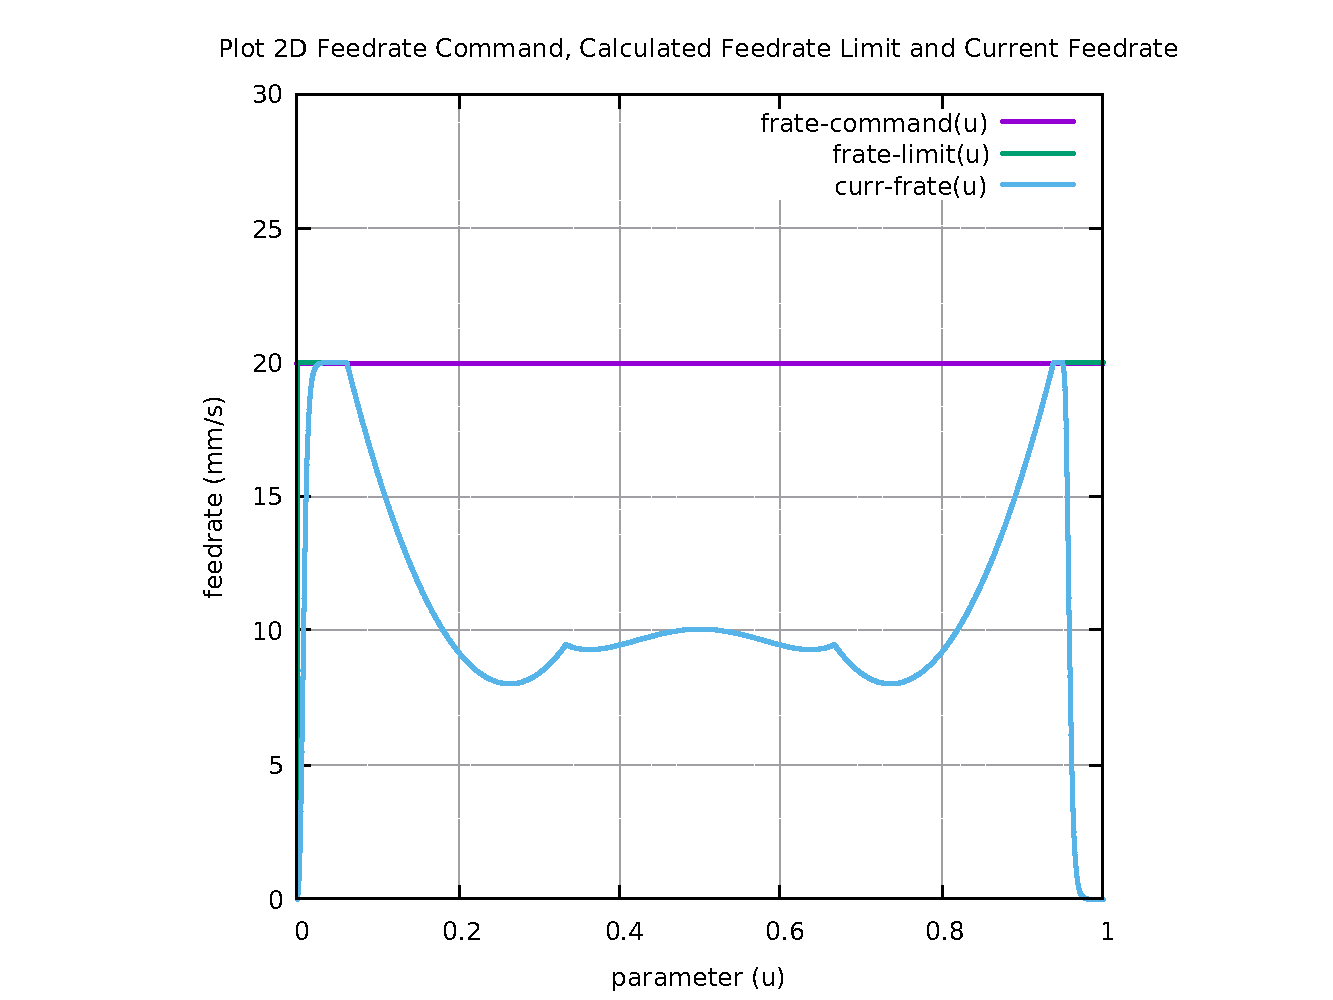
\includegraphics[width=1.00\textwidth]{Chap4/appendix/app-Teardrop/plots/11-img-Teardrop-FrateCommand-FrateLimit-and-Curr-Frate.pdf}
\end{figure}

\begin{figure}
	\caption     {Teardrop FeedRateLimit minus CurrFeedRate}
	\label{12-img-Teardrop-FeedRateLimit-minus-CurrFeedRate.pdf}
	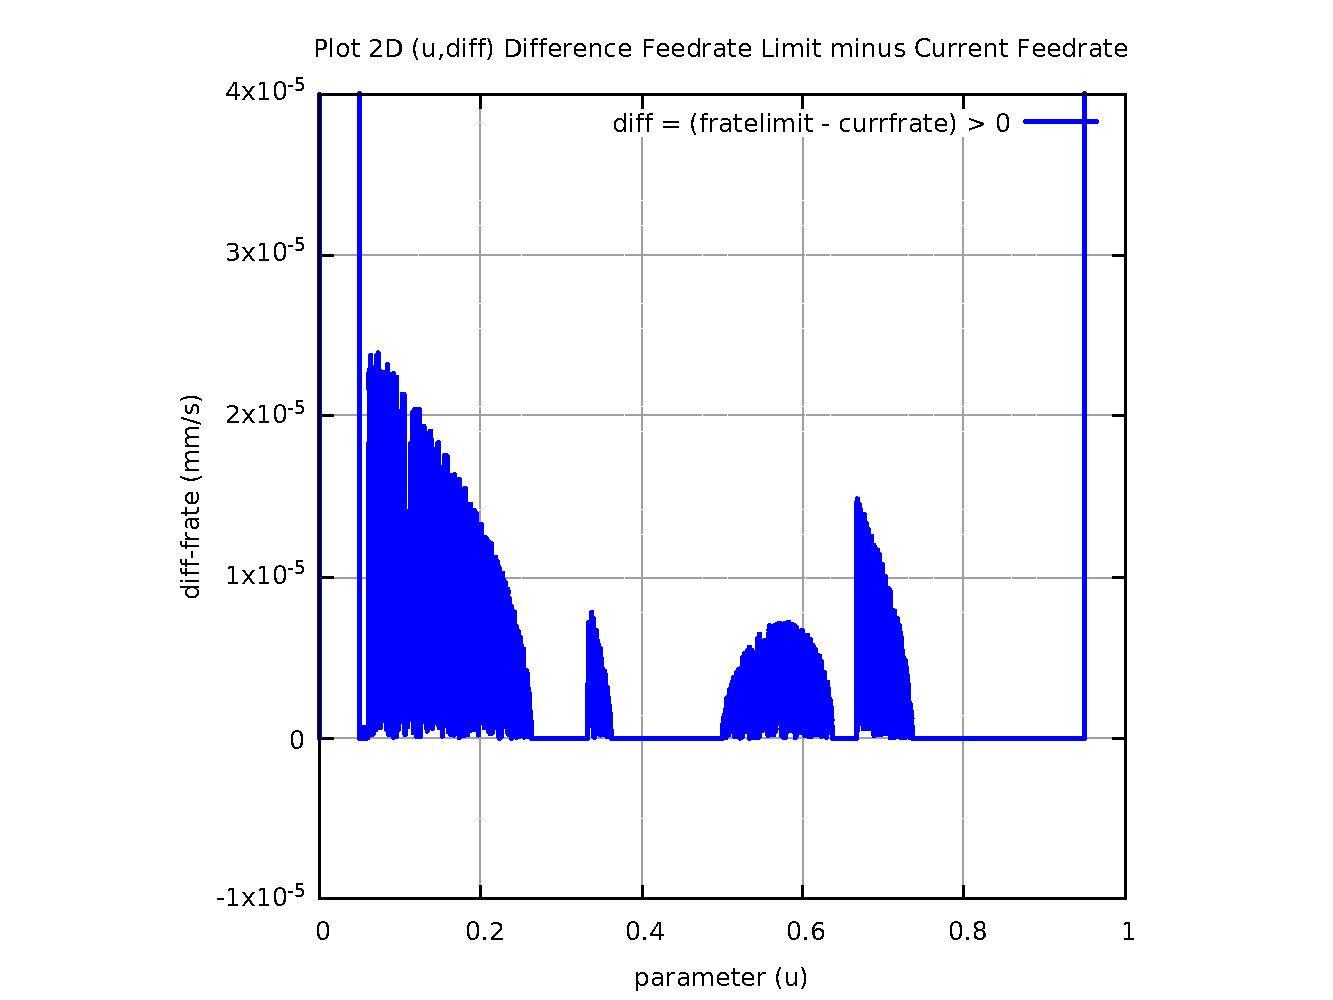
\includegraphics[width=1.00\textwidth]{Chap4/appendix/app-Teardrop/plots/12-img-Teardrop-FeedRateLimit-minus-CurrFeedRate.pdf}
\end{figure}

%% ==================================================
\clearpage
\pagebreak

\begin{figure}
	\caption     {Teardrop FC20-Nominal X and Y Feedrate Profiles}
	\label{13-img-Teardrop-FC20-Nominal-X-and-Y-Feedrate-Profiles.pdf}
	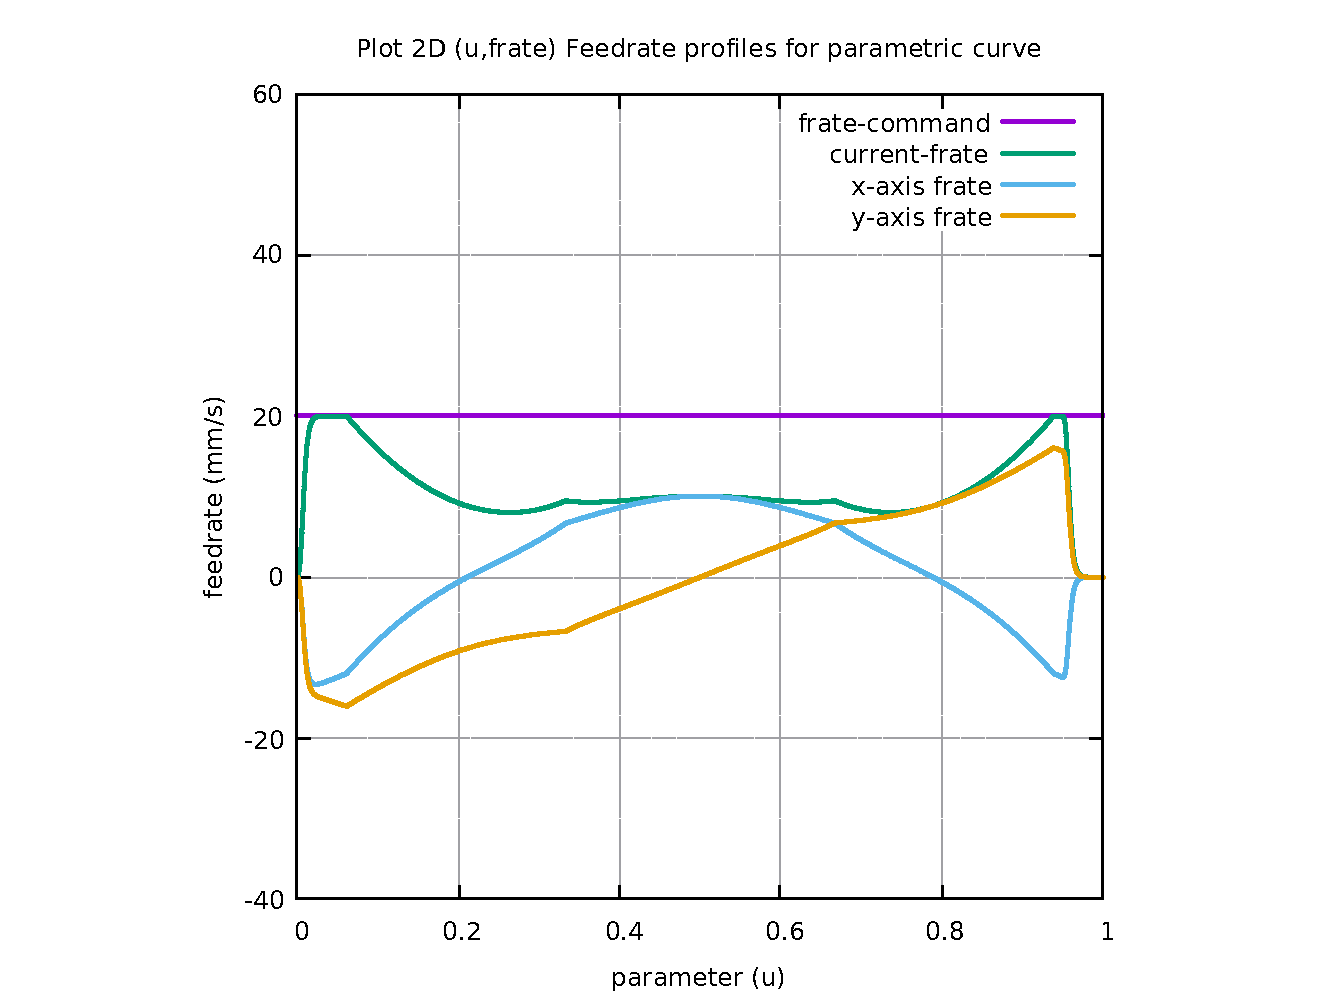
\includegraphics[width=1.00\textwidth]{Chap4/appendix/app-Teardrop/plots/13-img-Teardrop-FC20-Nominal-X-and-Y-Feedrate-Profiles.pdf}
\end{figure}


\begin{figure}
	\caption     {Teardrop FC20 Nominal Tangential Acceleration}
	\label{14-img-Teardrop-FC20-Nominal-Tangential-Acceleration.pdf}
	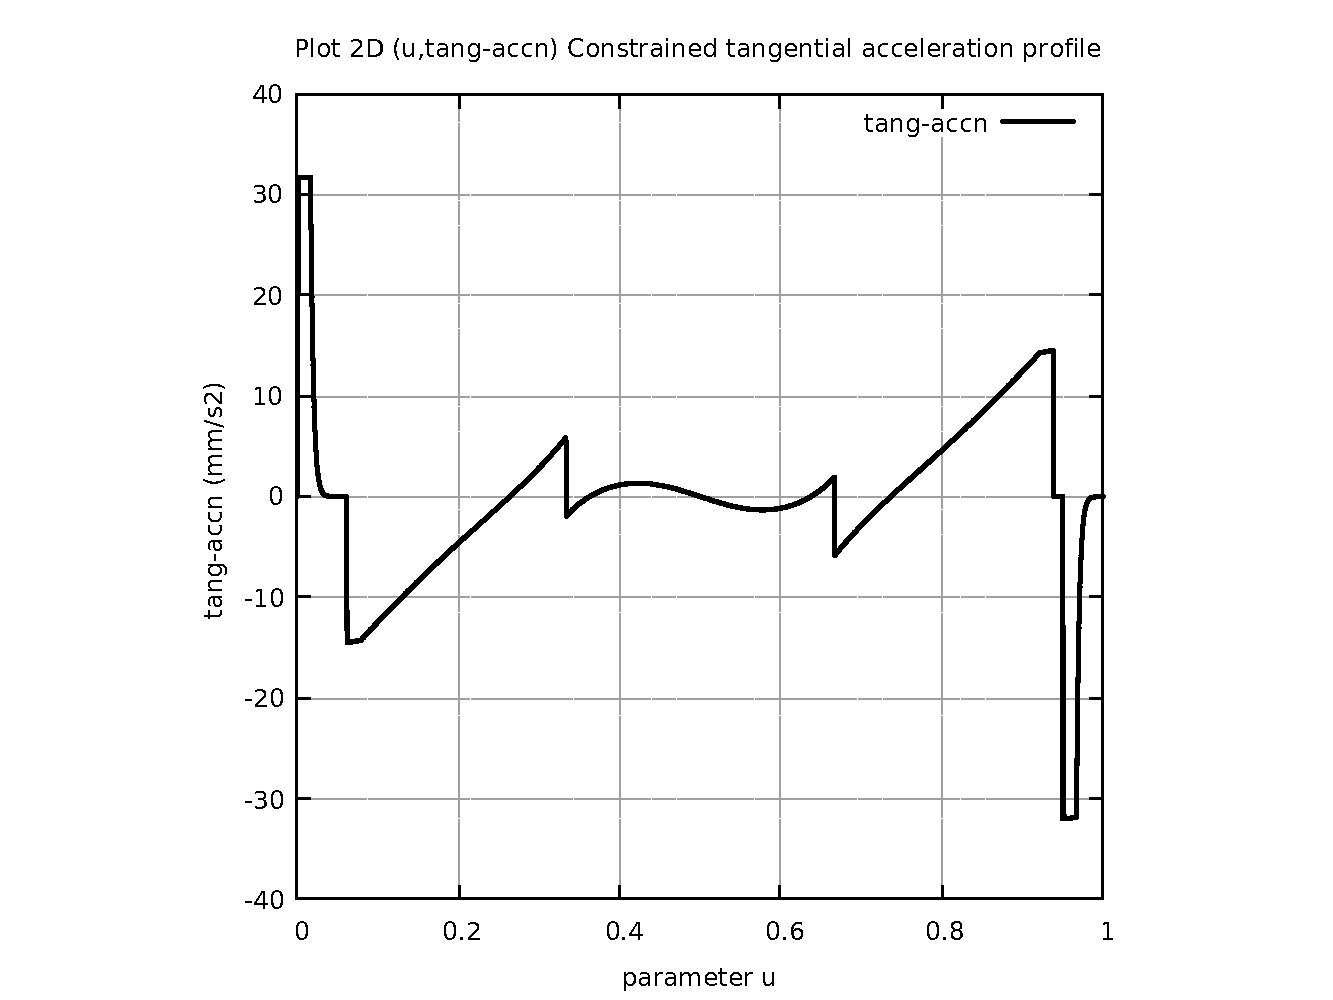
\includegraphics[width=1.00\textwidth]{Chap4/appendix/app-Teardrop/plots/14-img-Teardrop-FC20-Nominal-Tangential-Acceleration.pdf}
\end{figure}

%% ==================================================
\clearpage
\pagebreak

\begin{figure}
	\caption     {Teardrop FC20 Nominal Rising S-Curve Profile}
	\label{15-img-Teardrop-FC20-Nominal-Rising-S-Curve-Profile.pdf}
	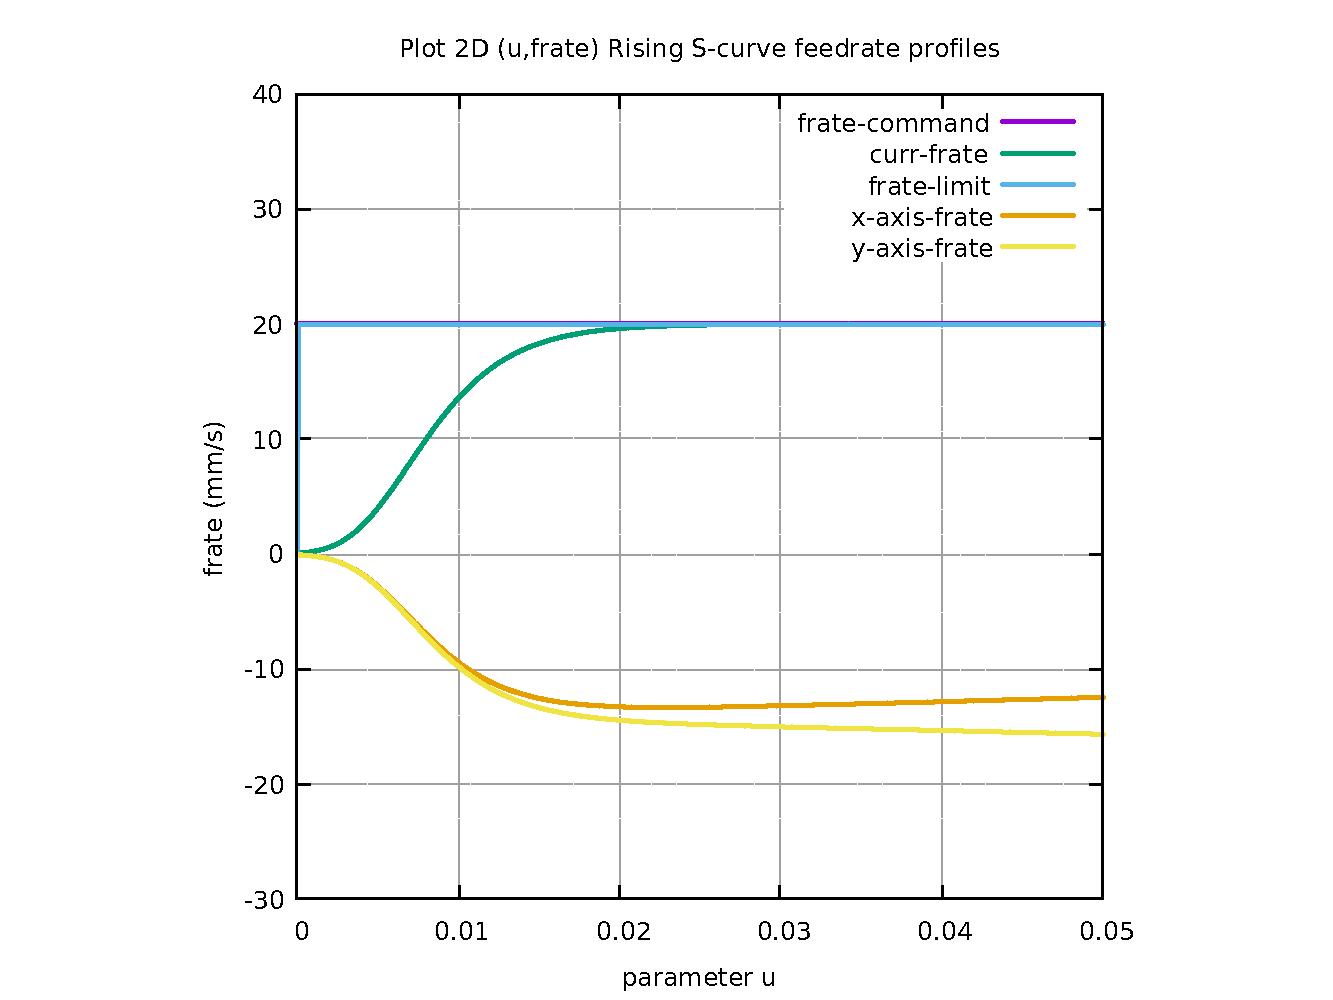
\includegraphics[width=1.00\textwidth]{Chap4/appendix/app-Teardrop/plots/15-img-Teardrop-FC20-Nominal-Rising-S-Curve-Profile.pdf}
\end{figure}


\begin{figure}
	\caption     {Teardrop FC20 Nominal Falling S-Curve Profile}
	\label{16-img-Teardrop-FC20-Nominal-Falling-S-Curve-Profile.pdf}
	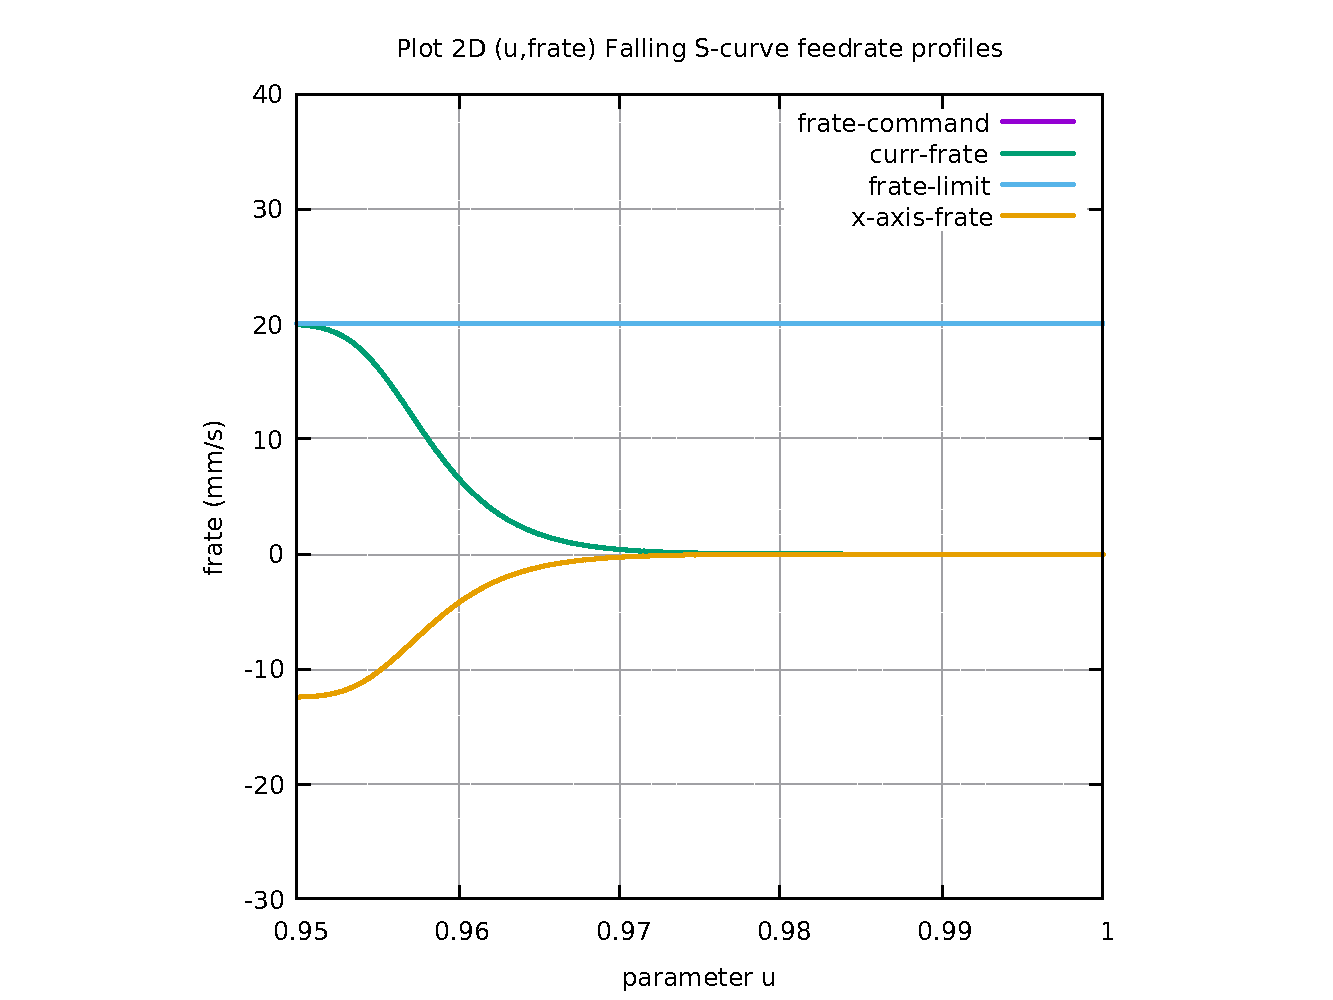
\includegraphics[width=1.00\textwidth]{Chap4/appendix/app-Teardrop/plots/16-img-Teardrop-FC20-Nominal-Falling-S-Curve-Profile.pdf}
\end{figure}

%% ==================================================
\clearpage
\pagebreak

\begin{figure}
	\caption     {Teardrop FC10 Colored Feedrate Profile data ngcode}
	\label{17-img-Teardrop-FC10-Colored-Feedrate-Profile-data_ngcode.png}
	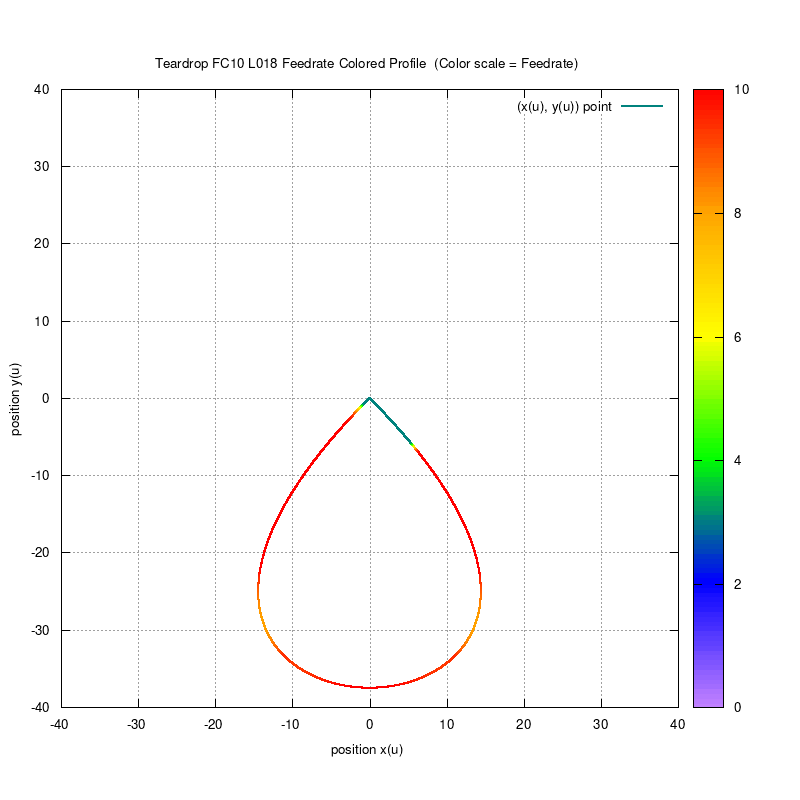
\includegraphics[width=0.75\textwidth]{Chap4/appendix/app-Teardrop/plots/17-img-Teardrop-FC10-Colored-Feedrate-Profile-data_ngcode.png}
\end{figure}


\begin{figure}
	\caption     {Teardrop FC20 Colored Feedrate Profile data ngcode}
	\label{18-img-Teardrop-FC20-Colored-Feedrate-Profile-data_ngcode.png}
	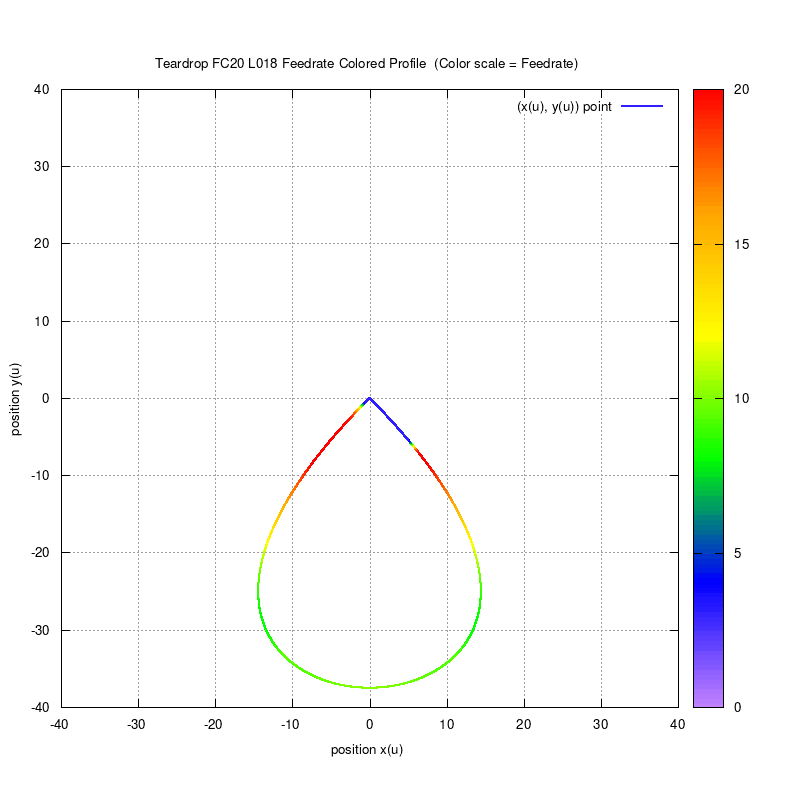
\includegraphics[width=0.75\textwidth]{Chap4/appendix/app-Teardrop/plots/18-img-Teardrop-FC20-Colored-Feedrate-Profile-data_ngcode.png}
\end{figure}

%% ==================================================
\clearpage
\pagebreak

\begin{figure}
	\caption     {Teardrop FC30 Colored Feedrate Profile data ngcode}
	\label{19-img-Teardrop-FC30-Colored-Feedrate-Profile-data_ngcode.png}
	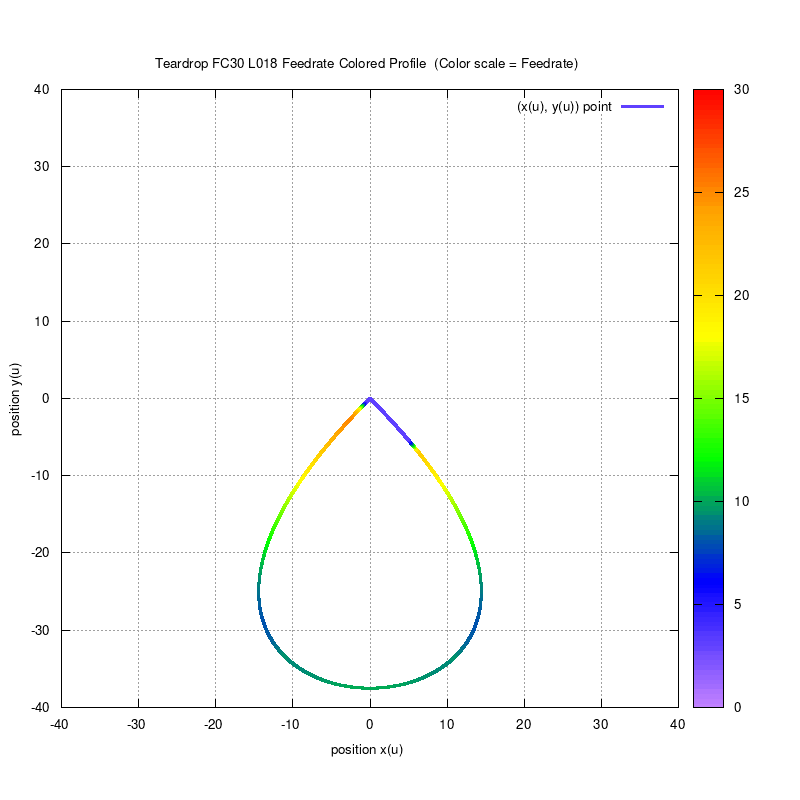
\includegraphics[width=0.75\textwidth]{Chap4/appendix/app-Teardrop/plots/19-img-Teardrop-FC30-Colored-Feedrate-Profile-data_ngcode.png}
\end{figure}


\begin{figure}
	\caption     {Teardrop FC40 Colored Feedrate Profile data ngcode}
	\label{20-img-Teardrop-FC40-Colored-Feedrate-Profile-data_ngcode.png}
	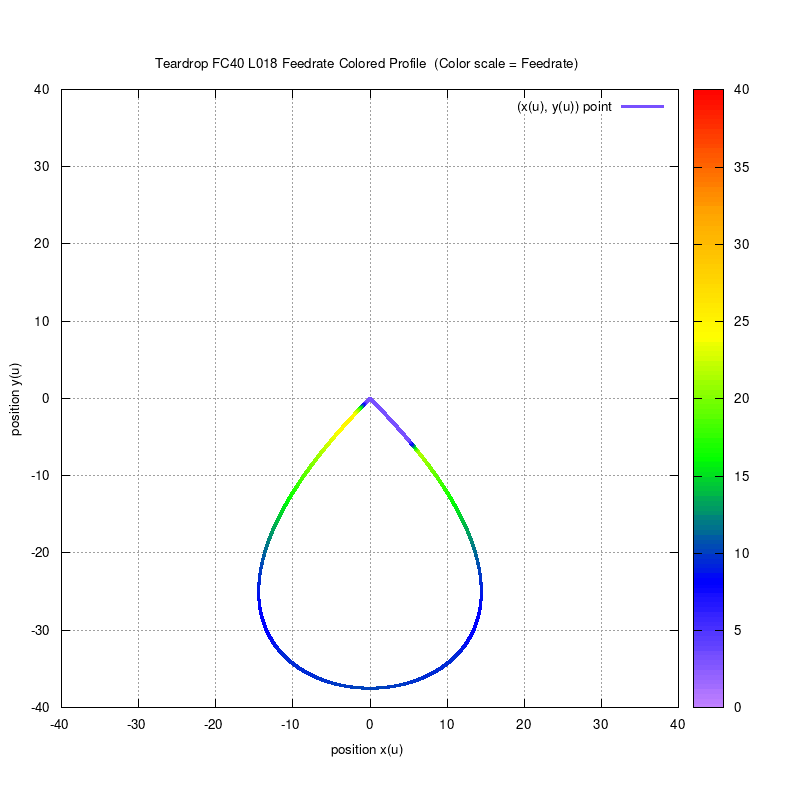
\includegraphics[width=0.75\textwidth]{Chap4/appendix/app-Teardrop/plots/20-img-Teardrop-FC40-Colored-Feedrate-Profile-data_ngcode.png}
\end{figure}

%% ==================================================
\clearpage
\pagebreak

\begin{figure}
	\caption     {Teardrop FC10 Tangential Acceleration}
	\label{21-img-Teardrop-FC10-Tangential-Acceleration.pdf}
	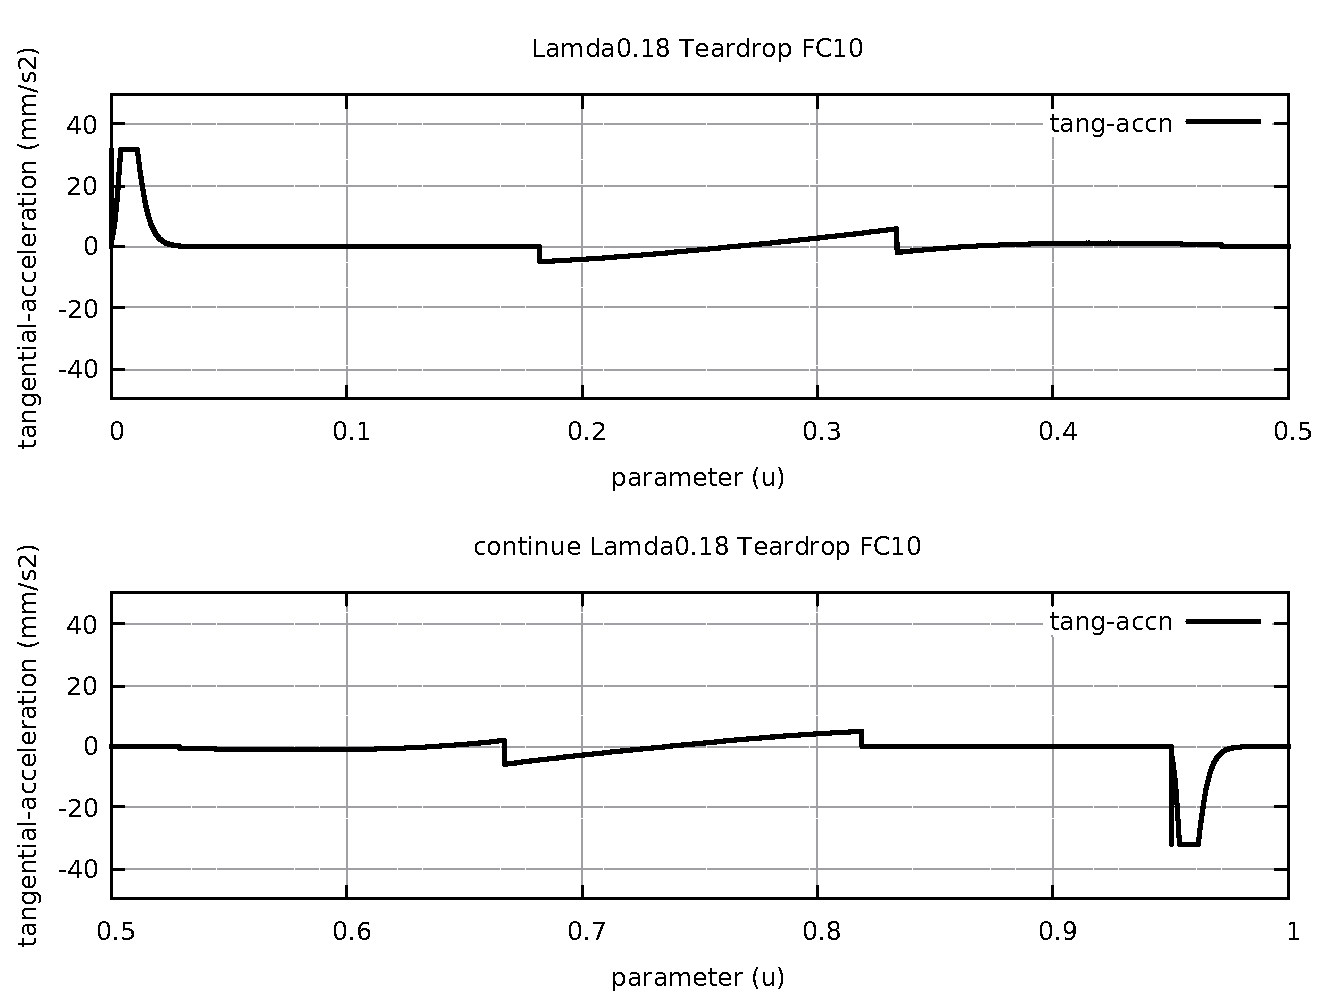
\includegraphics[width=1.00\textwidth]{Chap4/appendix/app-Teardrop/plots/21-img-Teardrop-FC10-Tangential-Acceleration.pdf}
\end{figure}


\begin{figure}
	\caption     {Teardrop FC20 Tangential Acceleration}
	\label{22-img-Teardrop-FC20-Tangential-Acceleration.pdf}
	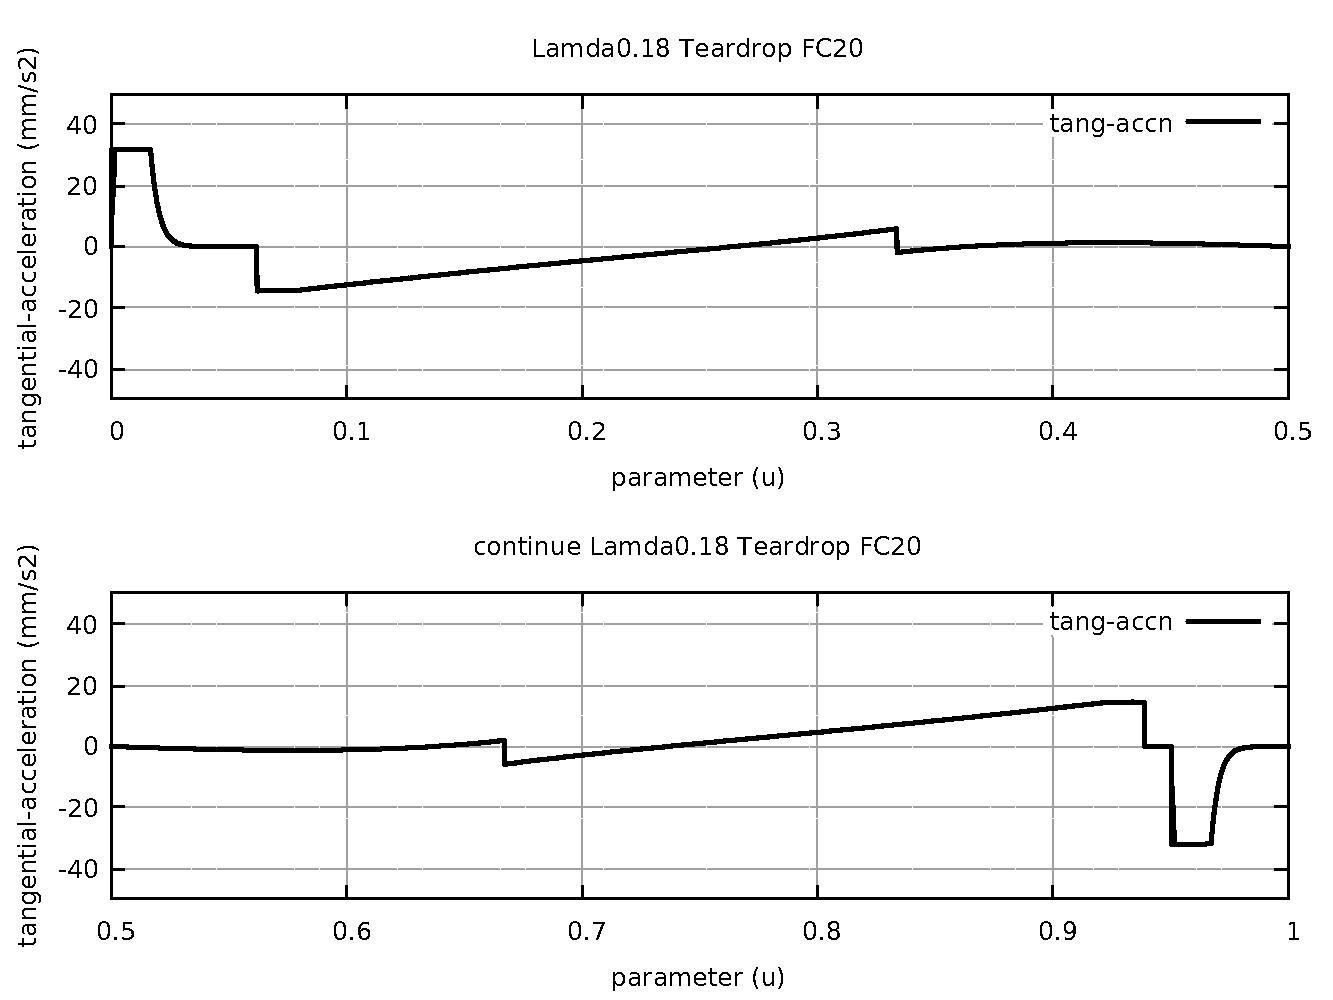
\includegraphics[width=1.00\textwidth]{Chap4/appendix/app-Teardrop/plots/22-img-Teardrop-FC20-Tangential-Acceleration.pdf}
\end{figure}

%% ==================================================
\clearpage
\pagebreak

\begin{figure}
	\caption     {Teardrop FC30 Tangential Acceleration}
	\label{23-img-Teardrop-FC30-Tangential-Acceleration.pdf}
	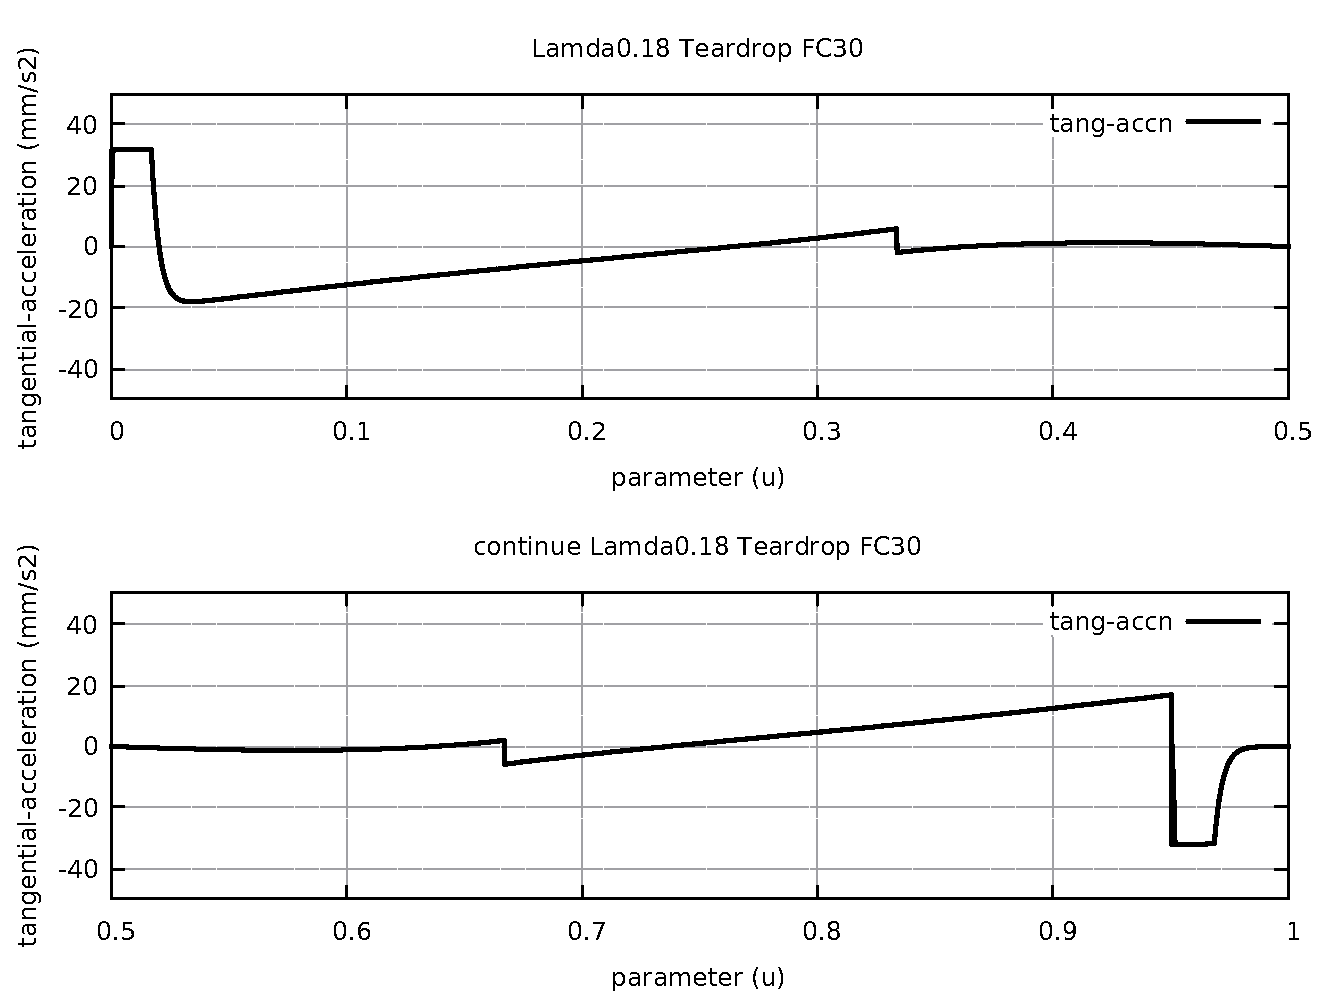
\includegraphics[width=1.00\textwidth]{Chap4/appendix/app-Teardrop/plots/23-img-Teardrop-FC30-Tangential-Acceleration.pdf}
\end{figure}


\begin{figure}
	\caption     {Teardrop FC40 Tangential Acceleration}
	\label{24-img-Teardrop-FC40-Tangential-Acceleration.pdf}
	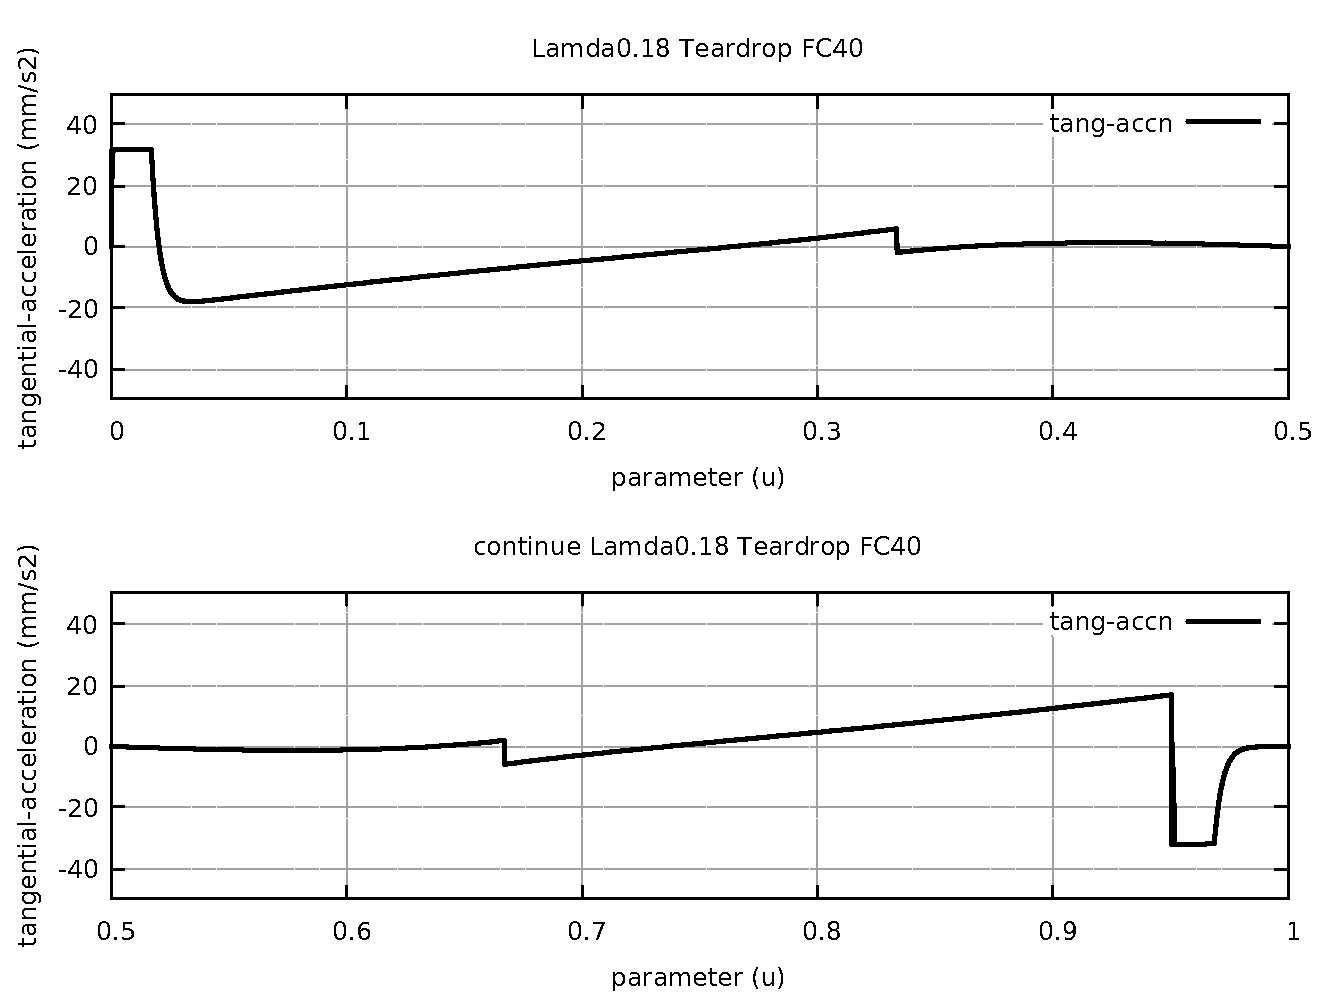
\includegraphics[width=1.00\textwidth]{Chap4/appendix/app-Teardrop/plots/24-img-Teardrop-FC40-Tangential-Acceleration.pdf}
\end{figure}

%% ==================================================
\clearpage
\pagebreak

\begin{figure}
	\caption     {Teardrop FC20 Nominal Separation NAL and NCL}
	\label{25-img-Teardrop-FC20-Nominal-Separation-NAL-and-NCL.pdf}
	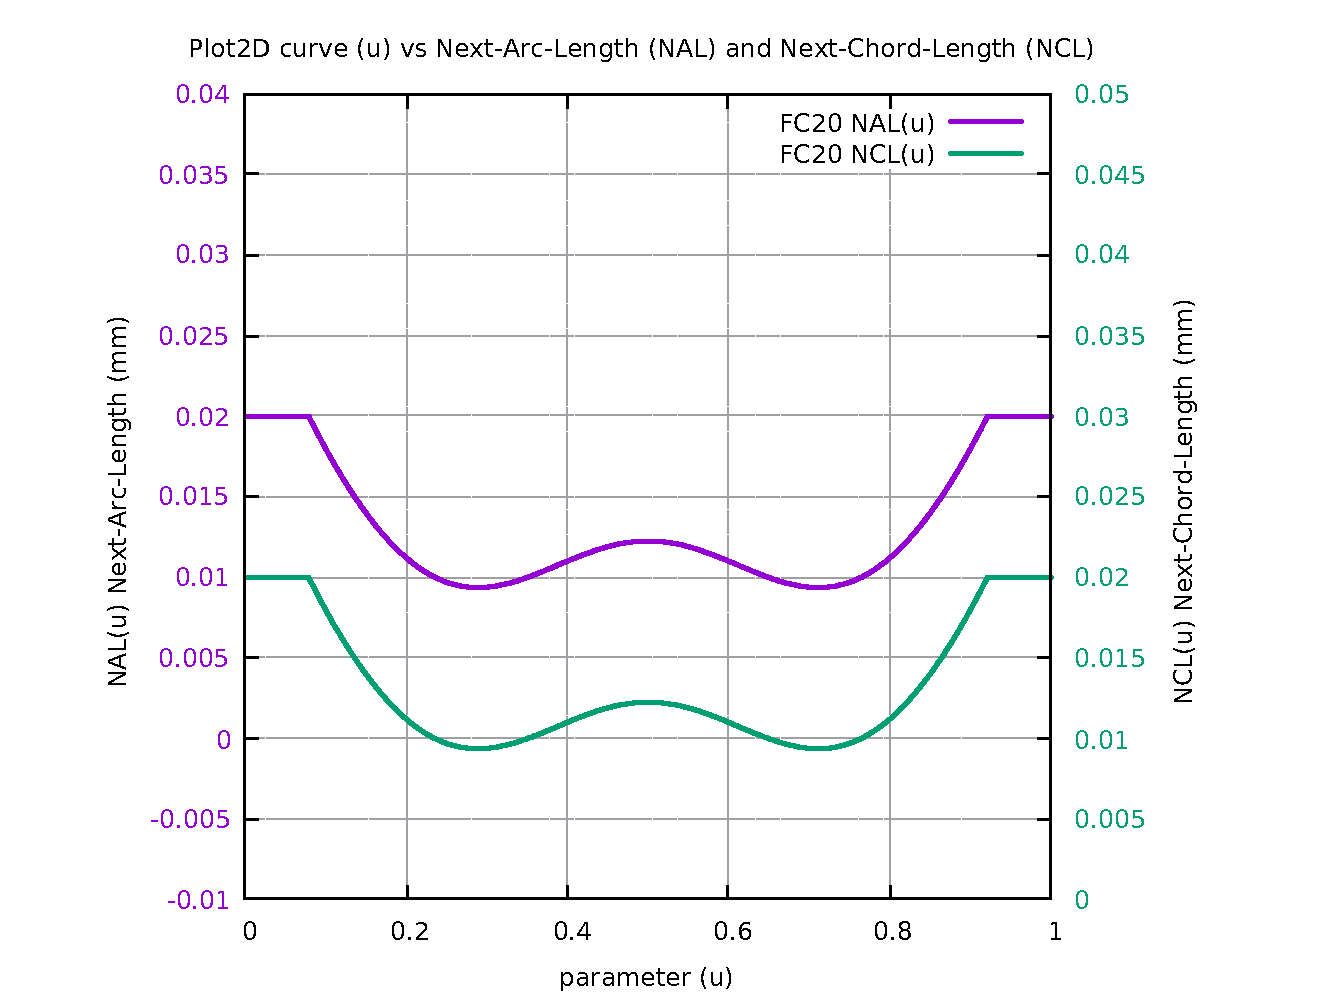
\includegraphics[width=1.00\textwidth]{Chap4/appendix/app-Teardrop/plots/25-img-Teardrop-FC20-Nominal-Separation-NAL-and-NCL.pdf}
\end{figure}


\begin{figure}
	\caption     {Teardrop Difference SAL minus SCL for FC10 FC20 FC30 FC40}
	\label{26-img-Teardrop-Difference-SAL-minus-SCL-for-FC10-FC20-FC30-FC40.pdf}
	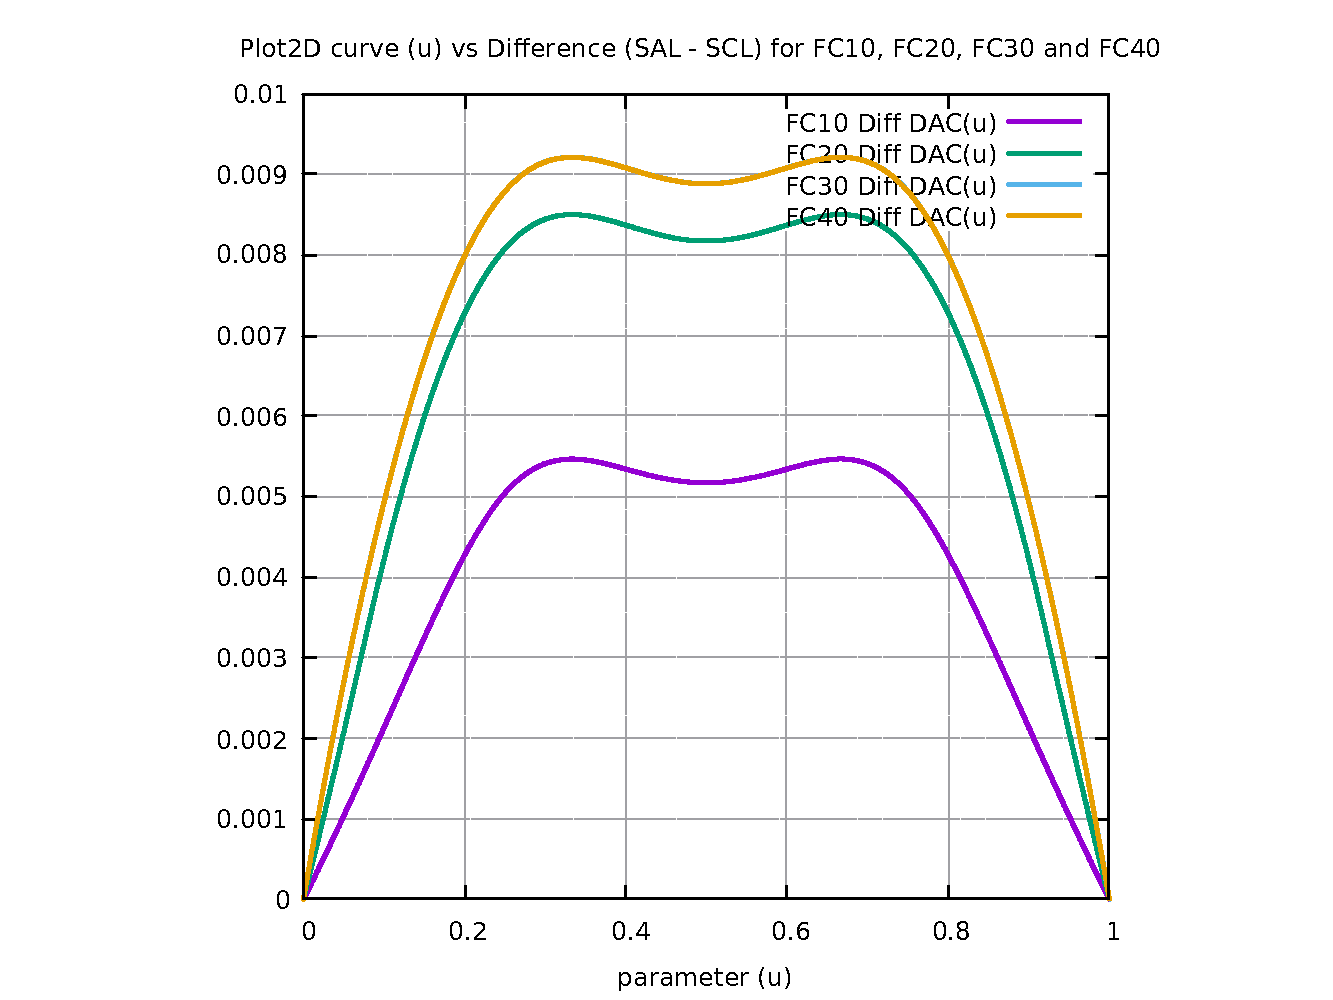
\includegraphics[width=1.00\textwidth]{Chap4/appendix/app-Teardrop/plots/26-img-Teardrop-Difference-SAL-minus-SCL-for-FC10-FC20-FC30-FC40.pdf}
\end{figure}


%% ==================================================
\clearpage
\pagebreak

\begin{figure}
	\caption     {Teardrop FC10 FrateCmd CurrFrate X-Frate Y-Frate}
	\label{27-img-Teardrop-FC10-FrateCmd-CurrFrate-X-Frate-Y-Frate.pdf}
	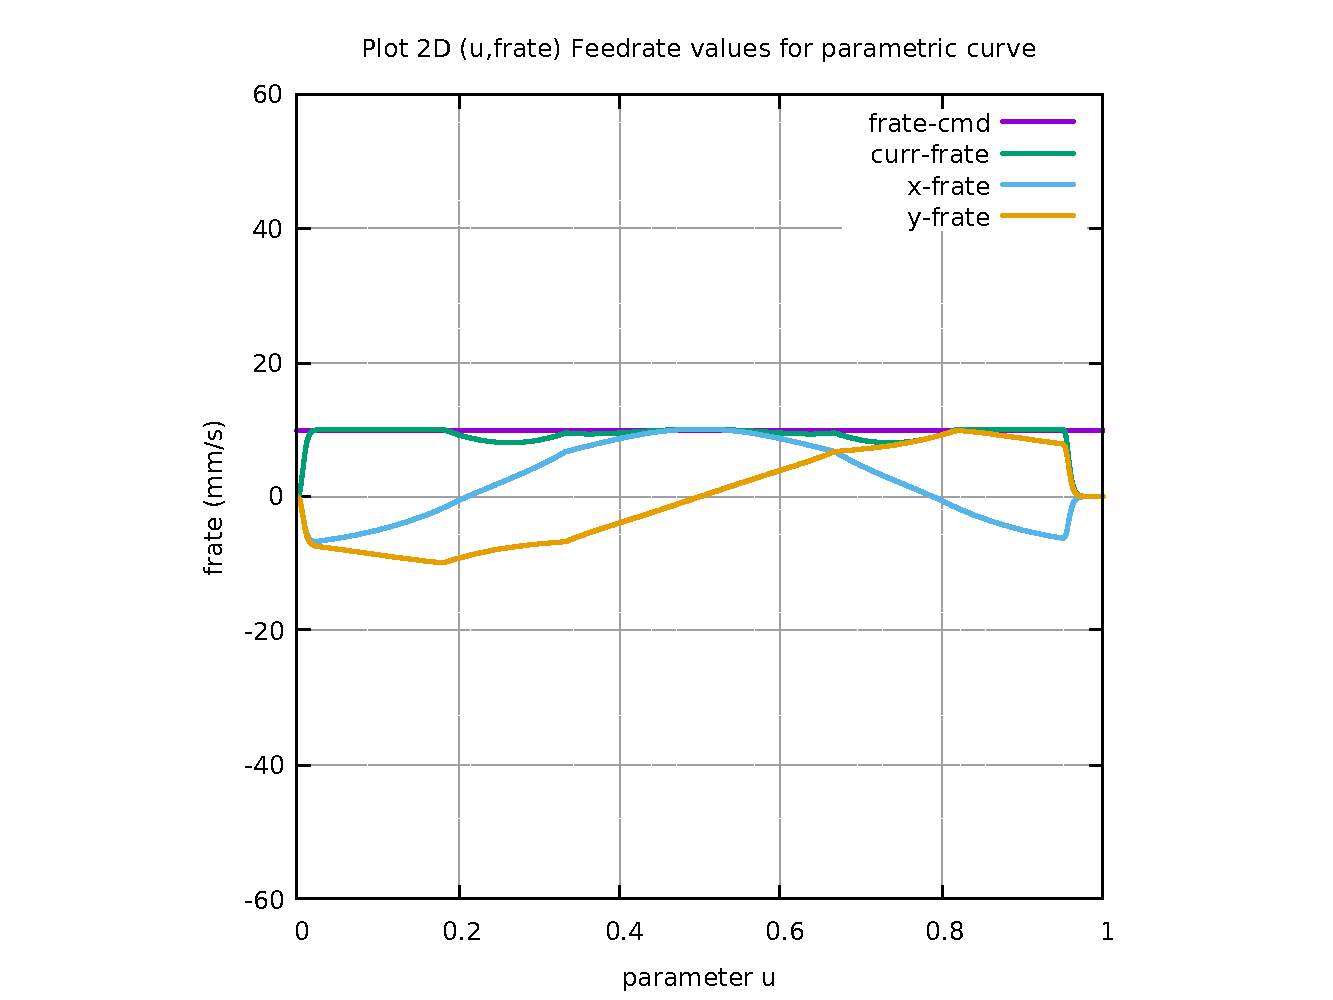
\includegraphics[width=1.00\textwidth]{Chap4/appendix/app-Teardrop/plots/27-img-Teardrop-FC10-FrateCmd-CurrFrate-X-Frate-Y-Frate.pdf}
\end{figure}


\begin{figure}
	\caption     {Teardrop FC20 FrateCmd CurrFrate X-Frate Y-Frate}
	\label{28-img-Teardrop-FC20-FrateCmd-CurrFrate-X-Frate-Y-Frate.pdf}
	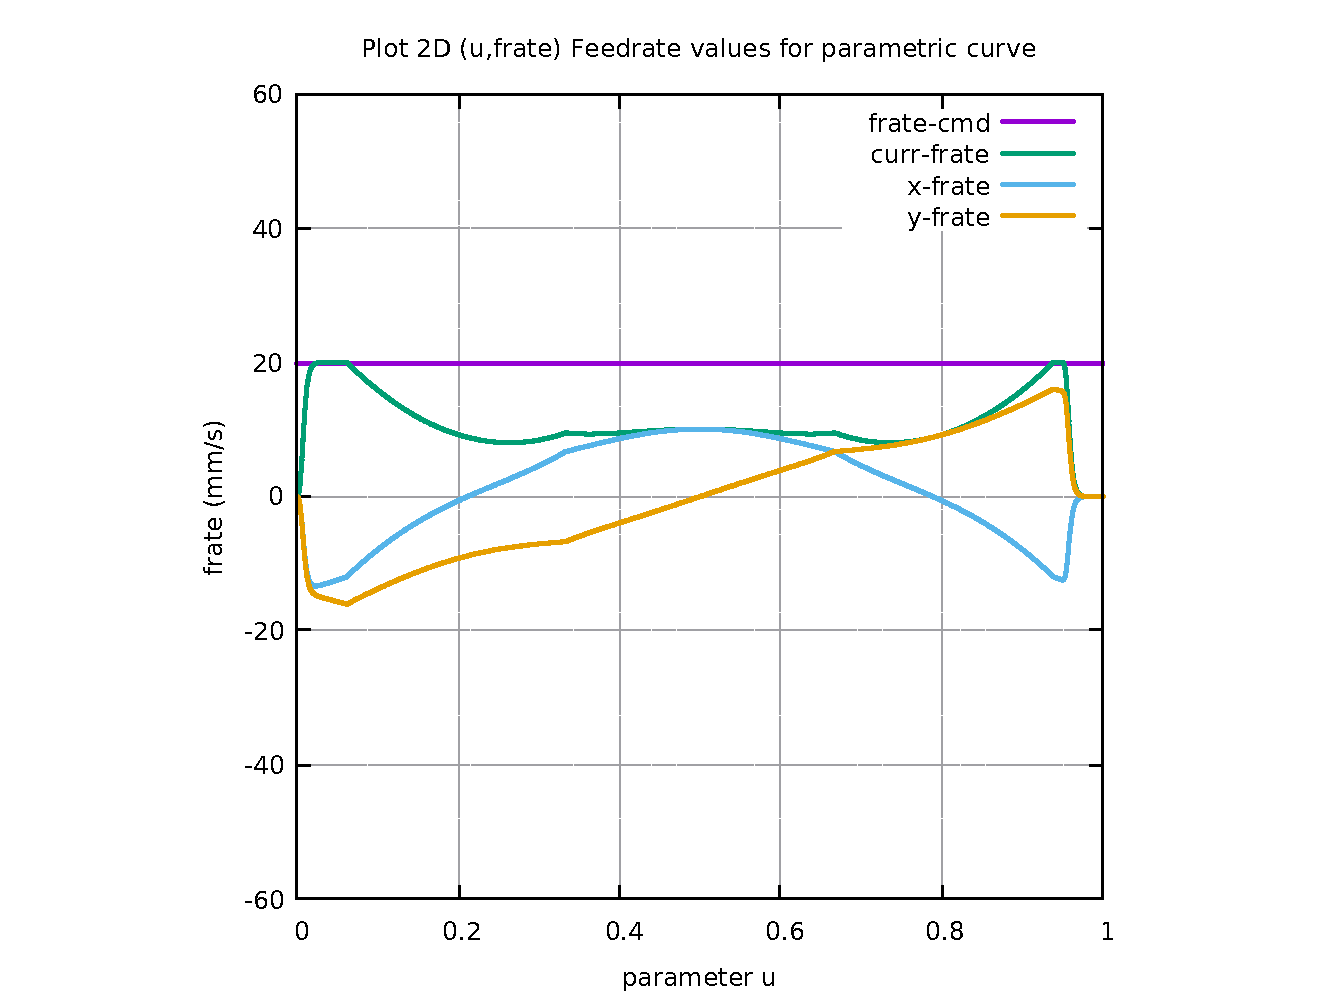
\includegraphics[width=1.00\textwidth]{Chap4/appendix/app-Teardrop/plots/28-img-Teardrop-FC20-FrateCmd-CurrFrate-X-Frate-Y-Frate.pdf}
\end{figure}


%% ==================================================
\clearpage
\pagebreak

\begin{figure}
	\caption     {Teardrop FC30 FrateCmd CurrFrate X-Frate Y-Frate}
	\label{29-img-Teardrop-FC30-FrateCmd-CurrFrate-X-Frate-Y-Frate.pdf}
	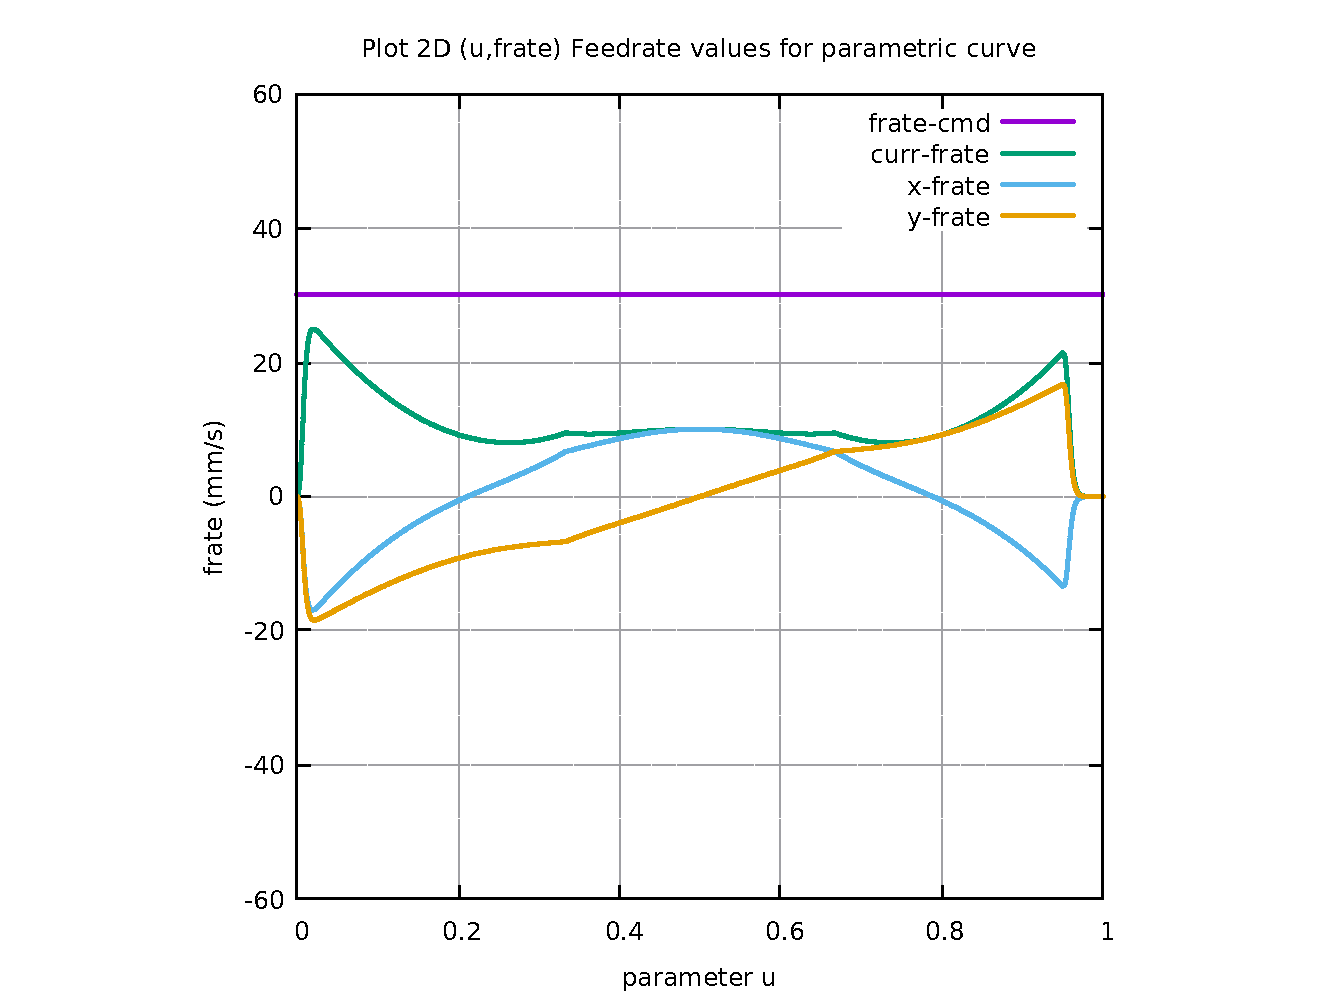
\includegraphics[width=1.00\textwidth]{Chap4/appendix/app-Teardrop/plots/29-img-Teardrop-FC30-FrateCmd-CurrFrate-X-Frate-Y-Frate.pdf}
\end{figure}


\begin{figure}
	\caption     {Teardrop FC40 FrateCmd CurrFrate X-Frate Y-Frate}
	\label{30-img-Teardrop-FC40-FrateCmd-CurrFrate-X-Frate-Y-Frate.pdf}
	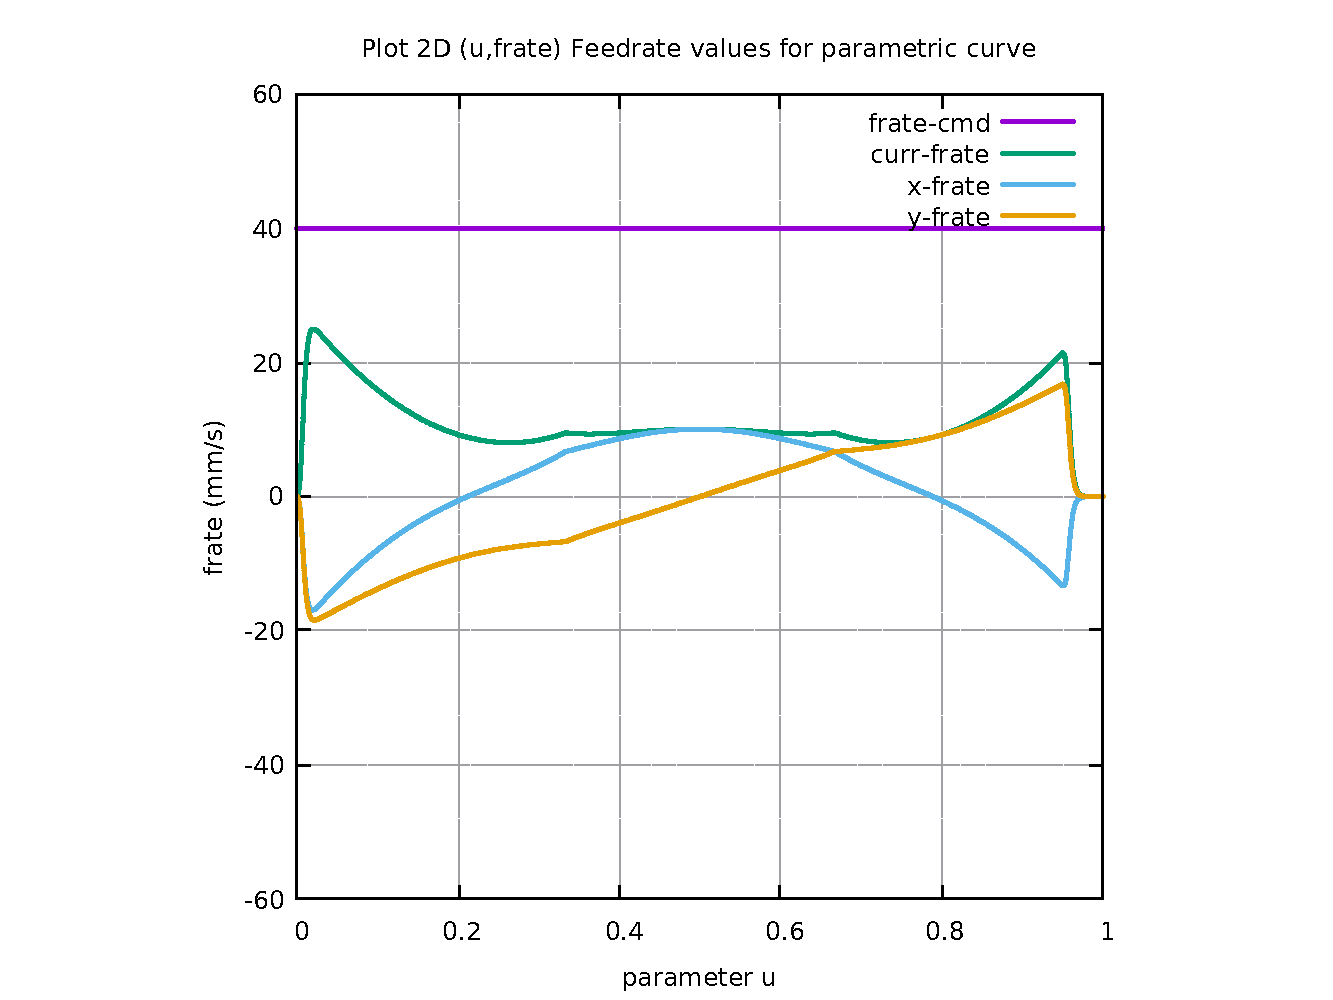
\includegraphics[width=1.00\textwidth]{Chap4/appendix/app-Teardrop/plots/30-img-Teardrop-FC40-FrateCmd-CurrFrate-X-Frate-Y-Frate.pdf}
\end{figure}


%% ==================================================
\clearpage
\pagebreak

\begin{figure}
	\caption     {Teardrop FC10 Four Components FeedrateLimit}
	\label{31-img-Teardrop-FC10-Four-Components-FeedrateLimit.pdf}
	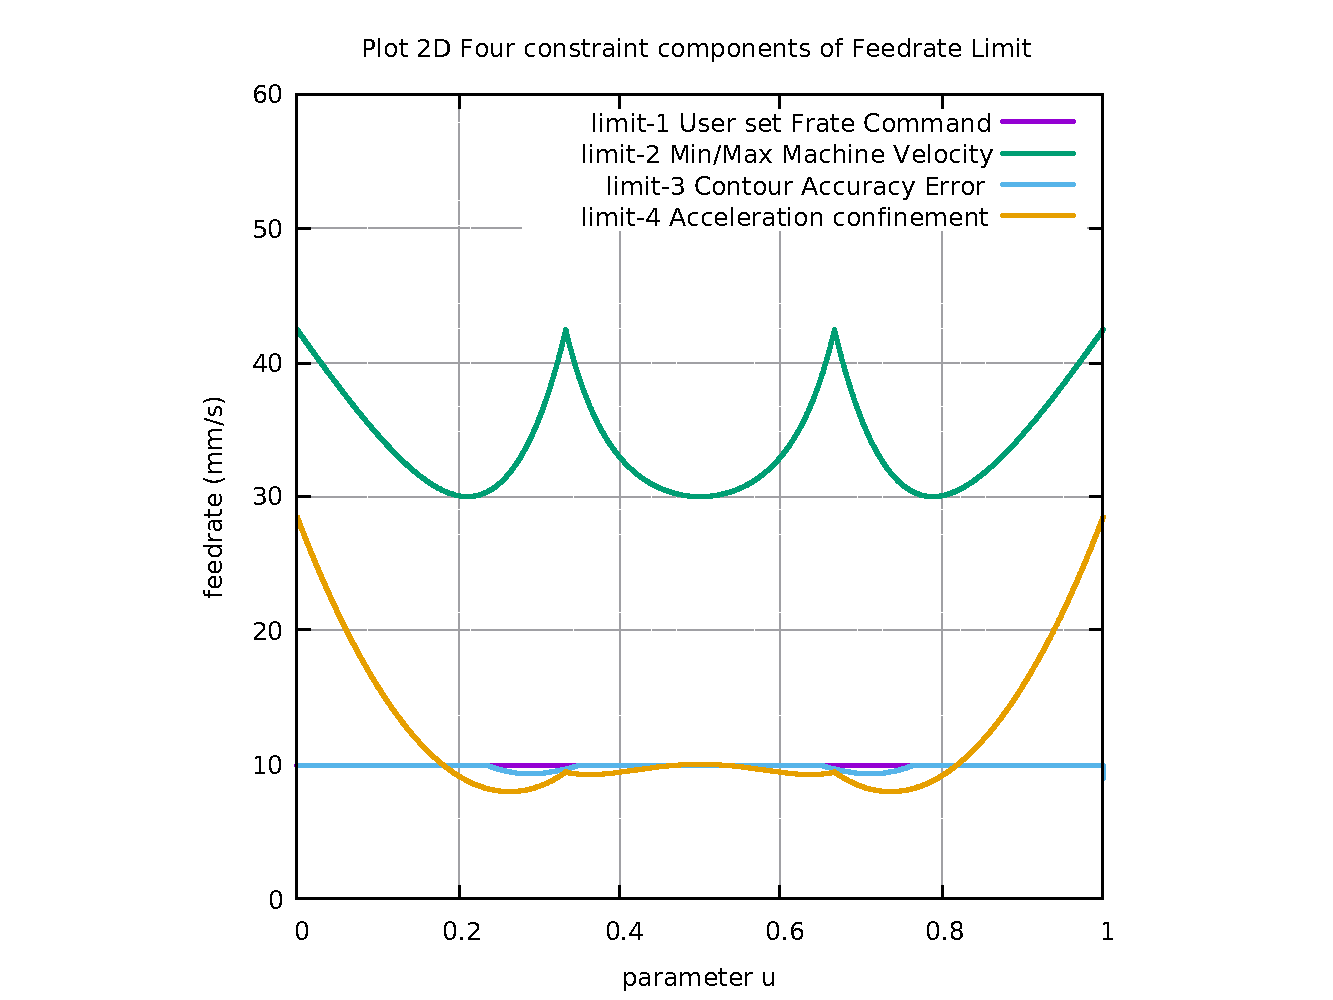
\includegraphics[width=1.00\textwidth]{Chap4/appendix/app-Teardrop/plots/31-img-Teardrop-FC10-Four-Components-FeedrateLimit.pdf}
\end{figure}


\begin{figure}
	\caption     {Teardrop FC20 Four Components FeedrateLimit}
	\label{32-img-Teardrop-FC20-Four-Components-FeedrateLimit.pdf}
	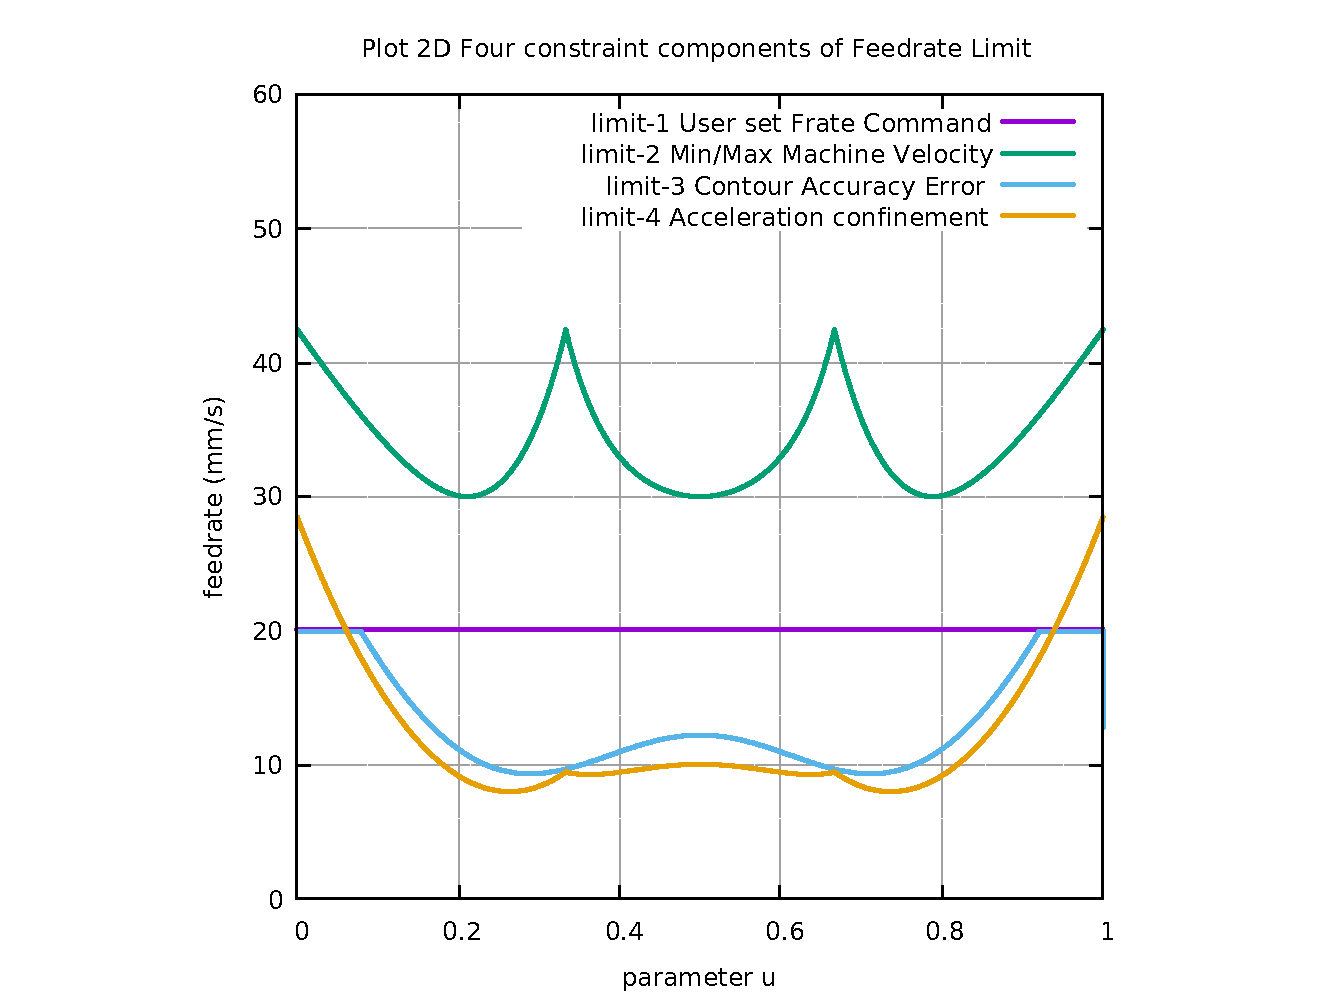
\includegraphics[width=1.00\textwidth]{Chap4/appendix/app-Teardrop/plots/32-img-Teardrop-FC20-Four-Components-FeedrateLimit.pdf}
\end{figure}


%% ==================================================
\clearpage
\pagebreak

\begin{figure}
	\caption     {Teardrop FC30 Four Components FeedrateLimit}
	\label{33-img-Teardrop-FC30-Four-Components-FeedrateLimit.pdf}
	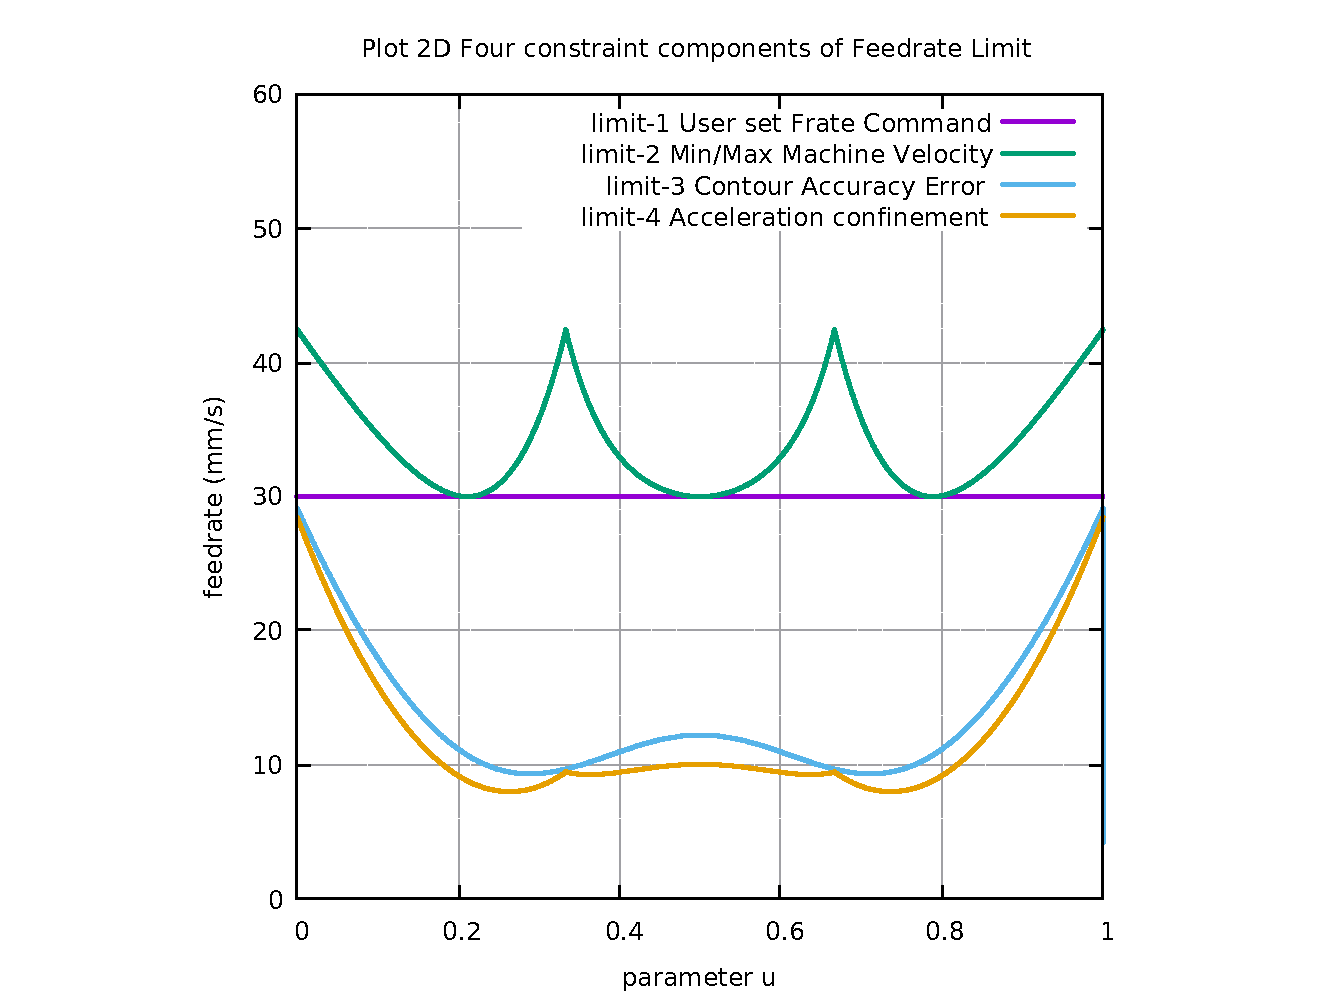
\includegraphics[width=1.00\textwidth]{Chap4/appendix/app-Teardrop/plots/33-img-Teardrop-FC30-Four-Components-FeedrateLimit.pdf}
\end{figure}


\begin{figure}
	\caption     {Teardrop FC40 Four Components FeedrateLimit}
	\label{34-img-Teardrop-FC40-Four-Components-FeedrateLimit.pdf}
	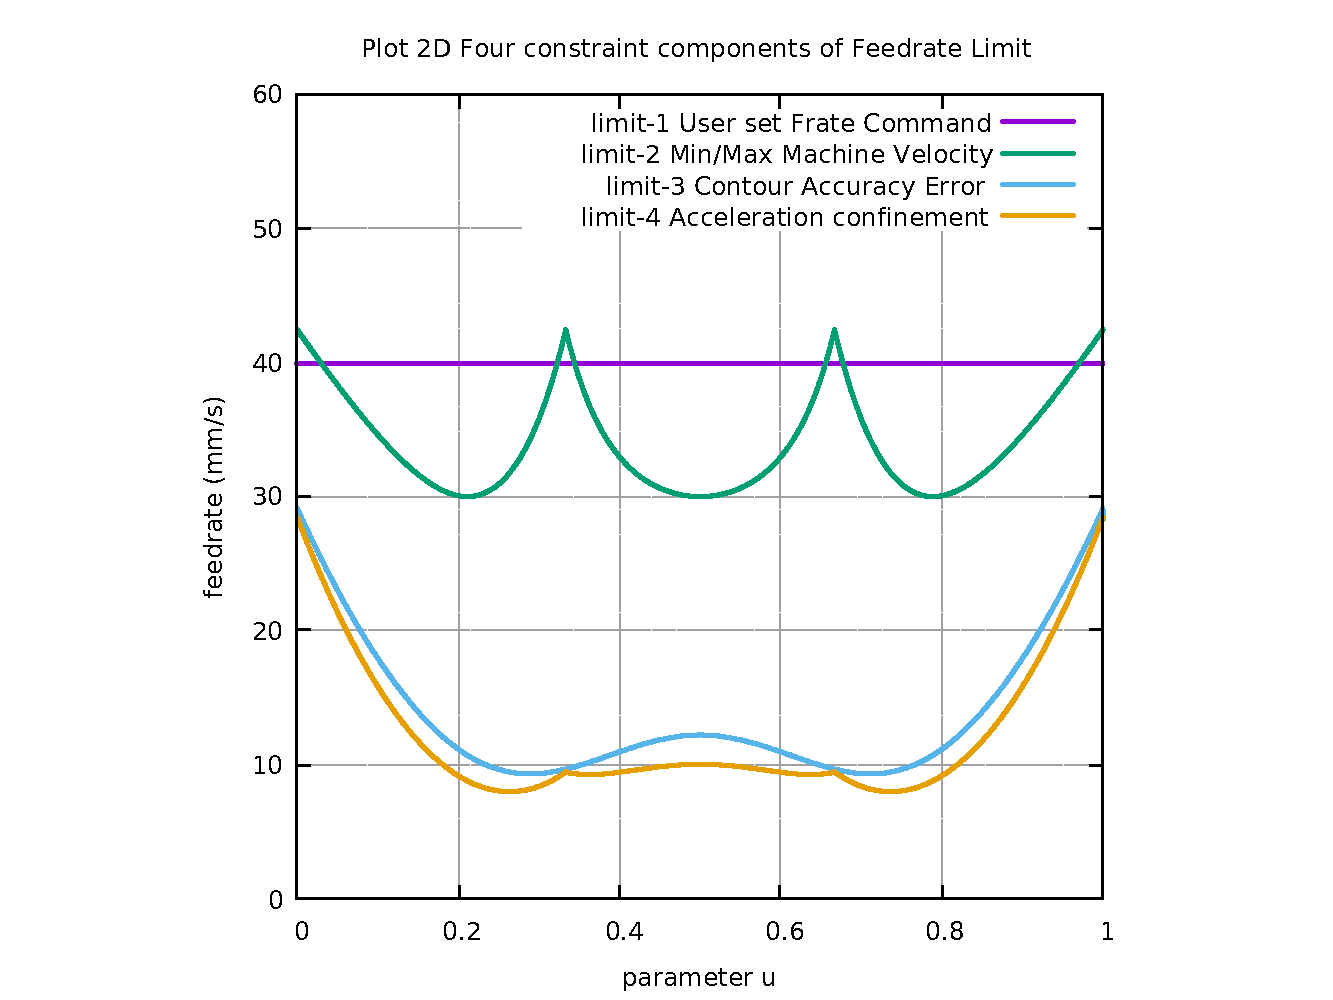
\includegraphics[width=1.00\textwidth]{Chap4/appendix/app-Teardrop/plots/34-img-Teardrop-FC40-Four-Components-FeedrateLimit.pdf}
\end{figure}


%% =======================================
\clearpage
\pagebreak

\begin{figure}
	\centering
	\caption     {Teardrop Histogram Points FC10 FC20 FC30 FC40}
	\label{35-img-Teardrop-Histogram-Points-FC10-FC20-FC30-FC40.pdf}
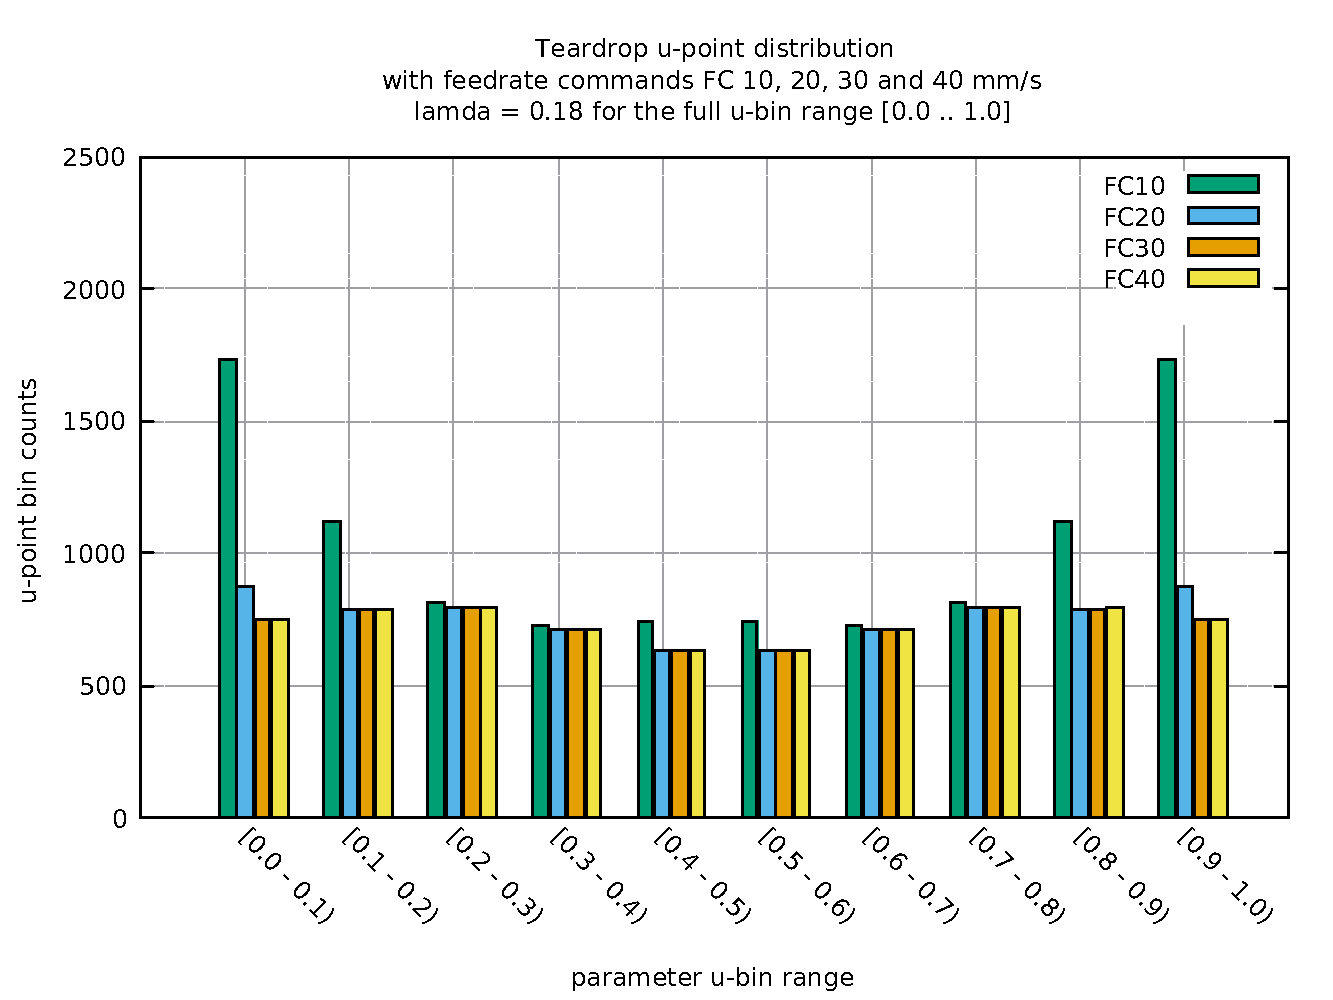
\includegraphics[width=1.00\textwidth]{Chap4/appendix/app-Teardrop/plots/35-img-Teardrop-Histogram-Points-FC10-FC20-FC30-FC40.pdf} 
\end{figure}


\begin{table}[ht]
	%% \begin{center}
\caption    {Teardrop Table distribution of interpolated points}
\label  {tab-Teardrop Table distribution of interpolated points}
	
%% IMPORTANT TO SCALEBOX BELOW
\scalebox{0.80}{
		
%% START COPY AND PASTE BELOW HERE
%% FROM \begin{tabular} UNTIL \end{tabular)
%% Note: adjust last p{} to get line width correct
		
		
\begin{tabular}{ p{4.5cm} p{1.5cm} p{1.5cm} p{1.5cm} p{7.50cm} }
	\hline
	&		    &		 &		  &	    \\
	BINS	    &	FC10 &  FC20  &  FC30  &  FC40  \\
	&		    &	     &		  &	     \\
	0.0 – 0.1	&	1734 &	875	  &	748	   &	748	\\
	0.1 – 0.2	&	1120 &	791	  &	791	   &	791	\\
	0.2 – 0.3	&	809	 &	794	  &	794	   &	794	\\
	0.3 – 0.4	&	726	 &	710	  &	711	   &	711	\\
	0.4 – 0.5	&	741	 &	629	  &	629	   &	629	\\
	0.5 – 0.6	&	742	 &	629	  &	628	   &	629	\\
	0.6 – 0.7	&	726	 &	710	  &	711	   &	711	\\
	0.7 – 0.8	&	809	 &	794	  &	794	   &	793	\\
	0.8 – 0.9   &	1120 &	791	  &	791	   &	792	\\
	0.9 – 1.0	&	1734 &	876	  &	750	   &	749	\\
	&		    &		 &		  &		\\
	Total counts&  10261 &	7599  &	7347   &   7347	\\
	&		    &		 &		  &		\\
\hline	
\end{tabular}
		
%% END COPY AND PASTE ABOVE HERE
}   %% IMPORTANT FOR SCALEBOX CLOSING
	

\end{table}
%% \end{landscape}

%% Teardrop SUMMARY TABLE
%% ========================================================
\clearpage
\pagebreak
\begin{landscape}
	
\begin{table}[ht]
%% \begin{center}
\caption       {Teardrop Table FC10-20-30-40 Run Performance data}
\label{tab-app4-Teardrop-Table-FC10-20-30-40-Run-Performance-data}
		
%% IMPORTANT TO SCALEBOX BELOW
\scalebox{0.90}{
			
%% START COPY AND PASTE BELOW HERE
%% FROM \begin{tabular} UNTIL \end{tabular)
			
			
\begin{tabular}{ p{0.2cm} p{8.80cm} p{4.00cm} p{4.0cm} p{4.00cm} p{4.0cm}}
	\hline
	&		&		&		&		&		\\
	1	&	Curve Type	&	TEARDROP	&	TEARDROP	&	TEARDROP	&	TEARDROP	\\
	2	&	User Feedrate Command FC(mm/s)                   	&	FC10	&	FC20	&	FC30	&	FC40	\\
	3	&	User Lamda Acceleration Safety Factor	&	0.18	&	0.18	&	0.18	&	0.18	\\
	&		&		&		&		&		\\
	4	&	Total Iterpolated Points (TIP)	&	10261	&	7599	&	7347	&	7347	\\
	5	&	Total Sum-Chord-Error (SCE) (mm)	&	5.809737838076E-03	&	7.140807162860E-03	&	7.336793707381E-03	&	7.335147000398E-03	\\
	6	&	Ratio 1 = (SCE/TIP) = Chord-Error/Point	&	5.662512512745E-07	&	9.398272128007E-07	&	9.987467611463E-07	&	9.985225973861E-07	\\
	&		&		&		&		&		\\
	7	&	Total Sum-Arc-Length (SAL) (mm)	&	1.018356741269E+02	&	1.018418663504E+02	&	1.018595636256E+02	&	1.018355644559E+02	\\
	8	&	Total Sum-Chord-Length (SCL) (mm)	&	1.018356732173E+02	&	1.018418655699E+02	&	1.018595666011E+02	&	1.018355608386E+02	\\
	9	&	Difference = (SAL – SCL) (mm)	&	9.095903408252E-07	&	7.805327442156E-07	&	-2.975420997586E-06	&	3.617250541765E-06	\\
	10	&	Percentage Difference = (SAL – SCL)/SAL	&	8.931942058845E-07	&	7.664163788301E-07	&	-2.921101261067E-06	&	3.552050367760E-06	\\
	&		&		&		&		&		\\
	11	&	Ratio 2 = (SCE/SCL) = Chord Error/Chord-Length	&	5.705012452441E-05	&	7.011661778683E-05	&	7.202851879506E-05	&	7.202932786929E-05	\\
	&		&		&		&		&		\\
	12	&	Total Sum-Arc-Theta (SAT) (rad)	&	4.712304324578E+00	&	4.712268805770E+00	&	4.712349787227E+00	&	4.712123379377E+00	\\
	13	&	Total Sum-Arc-Area (SAA) (mm2)	&	3.822127588087E-05	&	6.182290957317E-05	&	6.781012634326E-05	&	6.777759239889E-05	\\
	&		&		&		&		&		\\
	14	&	Ratio 3 = (SAA/SCL) = Arc-Area/Chord-Length	&	5.705012452441E-05	&	7.011661778683E-05	&	7.202851879506E-05	&	7.202932786929E-05	\\
	&		&		&		&		&		\\
	15	&	Average-Chord-Error (ACE) (mm)	&	5.662512512745E-07	&	9.398272128007E-07	&	9.987467611463E-07	&	9.985225973861E-07	\\
	16	&	Average-Arc-Length (AAL) (mm)	&	9.925504300871E-03	&	1.340377288107E-02	&	1.386599014779E-02	&	1.386272317668E-02	\\
	17	&	Average-Chord-Length (ACL) (mm)	&	9.925504212216E-03	&	1.340377277834E-02	&	1.386599055283E-02	&	1.386272268427E-02	\\
	18	&	Average-Arc-Theta (AAT) (rad)	&	4.592889205241E-04	&	6.201985793327E-04	&	6.414851330284E-04	&	6.414543124663E-04	\\
	19	&	Average-Arc-Area (AAA) (mm2)	&	3.725270553691E-09	&	8.136734610840E-09	&	9.230891143923E-09	&	9.226462346704E-09	\\
	&		&		&		&		&		\\
	20	&	Algorithm actual runtime on computer (ART) (s) 	&	4.487434922	&	19.907344569	&	28.094412173	&	32.96324077	\\
	&		&		&		&		&		\\
\hline	
\end{tabular}			

%% END COPY AND PASTE		
}   %% IMPORTANT FOR SCALEBOX CLOSING
		
\end{table}
\end{landscape}

%% =======================================
\clearpage
\pagebreak
